%!TEX TS-program = pdflatex
% video compile
% ffmpeg -r 15 -f image2 -s 1920x1080 -i frame-%d.png -vcodec libx264 -crf 25 -pix_fmt yuv420p filename.mp4

\documentclass[aspectratio=169]{beamer}

%packages
\usepackage{amsmath,amsthm,amssymb,amsfonts,amsxtra,amstext}
\usepackage{gensymb}
\usepackage{graphicx,float}
\usepackage{adjustbox}
\usepackage{media9} %needed for including movies, otherwise comment out
%various figure appearance tweaks:
\usepackage{subcaption}
\captionsetup[subfigure]{labelformat=empty,margin=1ex,justification=raggedright}
\captionsetup[figure]{labelformat=empty}
%table tweaks
\usepackage{multirow}
\usepackage{multicol}
%tikz stuff - can be safely commented out if not using tikz for anything
\usepackage{tikz}
\usetikzlibrary{tikzmark,fit,shapes.geometric,positioning,arrows,arrows.meta}
\tikzstyle{every picture}+=[remember picture]
\usepackage{animate}

%add your own graphics path as needed:
%\graphicspath{{../Common/Figures/}{../Common/Logos/}}

%presentation theme and Cornell branding
\usetheme{Frankfurt} %if you don't like the navigation links up top, switch to: \usetheme[]{Madrid}
\DefineNamedColor{named}{CornellRed}{cmyk}{0,1,0.79,0.2} 
\usecolortheme[named=CornellRed]{structure}
\usefonttheme[]{serif}
\setbeamertemplate{navigation symbols}{} %i find these useless. ymmv

%logos
\pgfdeclareimage[height=1.5cm]{culogo}{template/CULogored}
\pgfdeclareimage[height=0.625cm]{CULogowhite}{template/CULogowhite}
\pgfdeclareimage[height=1.5cm]{csilogo}{template/CSI_logo}
\pgfdeclareimage[height=1.5cm]{sioslogo}{template/SIOSLogo_color_vector}

%let's slap the Cornell logo on everything. branding!
\usepackage[absolute,overlay]{textpos}
\setlength{\TPHorizModule}{1mm}
\setlength{\TPVertModule}{1mm}
\newcommand{\MyLogo}{%
\begin{textblock}{14}(153.0,6.35)
  \pgfuseimage{CULogowhite}
\end{textblock}
}

%\BackgroundPicture creates a full-slide image 
%see below for usage example
\newcommand\BackgroundPicture[3]{%
    \setbeamertemplate{background}{%
    \parbox[c][\paperheight]{\paperwidth}{%
        %\vfill \hfill
 \includegraphics[width=#2\paperwidth,height=#3\paperheight]{#1}
         %\hfill \vfill
      }}}


%useful defs - add your own here
\def\mf{\mathbf}
\def\mb{\mathbb}
\def\mc{\mathcal}
\newcommand{\mfbar}[1]{\mf{\bar{#1}}}
\newcommand{\mfhat}[1]{\mf{\hat{#1}}}
\newcommand{\bdot}[1]{\ensuremath{\dot{\mathbf{#1}}}}
\newcommand{\bhat}[1]{\ensuremath{\hat{\mathbf{#1}}}}
\newcommand{\intd}[1]{\ensuremath{\,\mathrm{d}#1}}
\newcommand{\leftexp}[2]{{\vphantom{#2}}^{#1}\!{#2}}
\newcommand{\leftsub}[2]{{\vphantom{#2}}_{#1}\!{#2}}
\newcommand{\fddt}[1]{\ensuremath{\leftexp{\mathcal{#1}}{\frac{\mathrm{d}}{\mathrm{d}t}}}}
\newcommand{\fdddt}[1]{\ensuremath{\leftexp{\mathcal{#1}}{\frac{\mathrm{d}^2}{\mathrm{d}t^2}}}}
\newcommand{\omegarot}[2]{\ensuremath{\leftexp{\mathcal{#1}}{\boldsymbol{\omega}}^{\mathcal{#2}}}}
\newcommand{\refeq}[1]{Equation  (\ref{#1})} 
\newcommand{\reftable}[1]{Table \ref{#1}}  
\newcommand{\reffig}[1]{Figure \ref{#1}}
\newcommand{\refnum}[1]{Ref.~\citenum{#1}}

%fonts and colors - add own defs here
\setbeamerfont{smalleq}{size=\tiny} 
\definecolor{MyBlue}{cmyk}{0.88, 0.7637,0.0032,0} 
\definecolor{MyRed}{cmyk}{0,0.994,1,0} 
\definecolor{MyGreen}{cmyk}{0.8985,0.3258,1,0.2429} 
\definecolor{MyPurple}{cmyk}{0.7708,0.847,0,0} 
\definecolor{MyGraphite}{cmyk}{0.5973,0.5124,0.5077,0.2013} 

% presentation descriptors
\title[]{Scheduling Direct Imaging Observations of Exoplanets Based on Radial Velocity Data}
\subtitle[]{Best Practices and Failure Modes}
\author[]{Corey Spohn}
%if you don't want logos on the title page (or don't want all of them, modify this:
\institute[]{\pgfuseimage{culogo}\hspace{0.75cm}\pgfuseimage{csilogo}\hspace{0.75cm}\pgfuseimage{sioslogo}}
\date[]{10/13/2021}
\subject{Talks} %modify as desired

%bib stuff 
%\usepackage[backend=biber, style=authoryear-comp]{biblatex}
\usepackage[style=authoryear]{biblatex}
\addbibresource{library.bib} %change to your own bibliography file

%custom cite command - change at will (change tiny to footnotesize to make bigger)
\newcommand{\customcite}[1]{\tiny{\citeauthor{#1}, \citetitle{#1}, \citeyear{#1}}}
\newcommand{\customcitenorm}[1]{{\citeauthor{#1}, \citetitle{#1}, \citeyear{#1}}}

% add a macro that saves its argument
\makeatletter
\newcommand{\footlineextra}[1]{\gdef\insertfootlineextra{#1}}
\newbox\footlineextrabox

% add a beamer template that sets the saved argument in a box.
% The * means that the beamer font and color "footline extra" are automatically added. 
\defbeamertemplate*{footline extra}{default}{
    \begin{beamercolorbox}[ht=2.25ex,dp=1ex,leftskip=1ex,wd=0.95\paperwidth]{footline extra}
    \insertfootlineextra
    %\par\vspace{2.5pt}
    \end{beamercolorbox}
}

\addtobeamertemplate{footline}{%
    % set the box with the extra footline material but make it add no vertical space
    \setbox\footlineextrabox=\vbox{\usebeamertemplate*{footline extra}}
    \vskip -\ht\footlineextrabox
    \vskip -\dp\footlineextrabox
    \box\footlineextrabox%
}

% patch \begin{frame} to reset the footline extra material
\let\beamer@original@frame=\frame
\def\frame{\gdef\insertfootlineextra{}\beamer@original@frame}
\footlineextra{}
\makeatother

%record left margin for making things full-frame
\makeatletter
\newlength\beamerleftmargin
\setlength\beamerleftmargin{\Gm@lmargin}
\makeatother
\graphicspath{{./}{figures/}}

\beamertemplategridbackground[10pt]

% TikZ stuff
\tikzset{
  every overlay node/.style={
    draw=none,fill=none,anchor=north west,inner sep=0, outer sep=0,
  },
}
% Usage:
% \tikzoverlay at (-1cm,-5cm) {content};
% or
% \tikzoverlay[text width=5cm] at (-1cm,-5cm) {content};
\def\tikzoverlay{%
   \tikz[baseline,overlay]\node[every overlay node]
}%
\usetikzlibrary{decorations.pathreplacing,calc,tikzmark}

\AtBeginSection[]{
  \begin{frame}
  \vfill
  \centering
  \begin{beamercolorbox}[sep=8pt,center,shadow=true,rounded=true]{title}
    \usebeamerfont{title}\insertsectionhead\par%
  \end{beamercolorbox}
  \vfill
  \end{frame}
}
\usepackage{colortbl}

\begin{document}

\part{Talk}
\frame[plain]{\titlepage
\vfill
\centering
%{\tiny You may wish to put auspices statements here, or not}
}

%after the title page, set up slide appearance
\setbeamertemplate{background}{ \setbeamercolor{normal text}{bg=white} }
\addtobeamertemplate{headline}{}{\MyLogo}
\setbeamertemplate{navigation symbols}{\insertframenumber{}/\inserttotalframenumber}
\beamertemplategridbackground[1cm]

%%%%%%%%%%%%%%%%%%%%%%%%%%%%%%%%%%%%%%%%%%%%%%%%%%%%%%%%%%%%%%%%%%%%%%%%%%%%%%%%%%%%%%%%%%%%%
\section{Intro}
\subsection{Intro}

\frame{
\frametitle{Exoplanet exploration}
\tikzoverlay[text width = 8cm] at (0cm, 3cm+4.5pt){
\begin{itemize}
    \item[\textbullet]  NASA's Exoplanet Exploration Program's primary goal is to ``discover and characterize
        planetary systems and Earth-like planets around nearby stars''
    \item[\textbullet] Further, the program is looking for signs of possible life which is studied through
        atmospheric characterization
    \item[\textbullet] To make detailed atmospheric characterization we need light from an exoplanet, either via
        transmission spectroscopy or direct imaging.
\end{itemize}
};
\tikzoverlay[text width = 5cm] at (8.35cm, 1.65cm){
    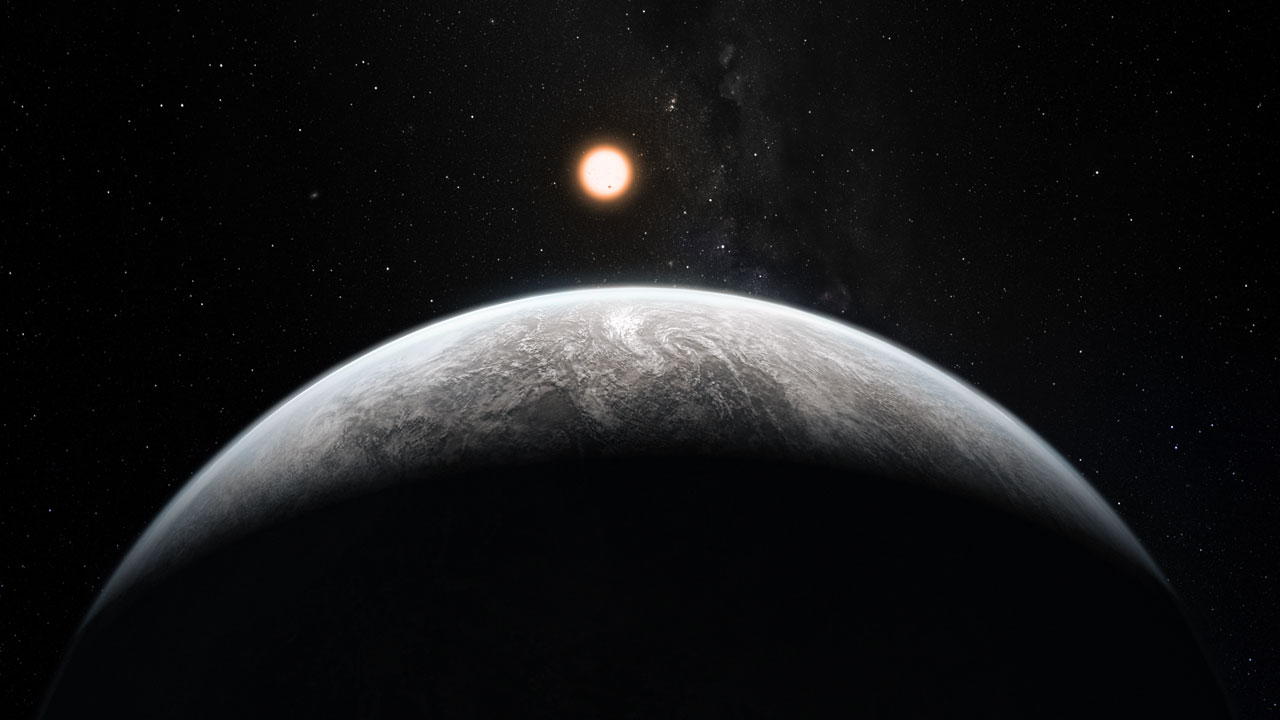
\includegraphics[width=6cm]{figures/exoplanet_art.jpeg}
};
\footlineextra{https://exoplanets.nasa.gov/system/internal\_resources/details/original/852\_Super\_Earth.jpeg}
}

\frame{
\frametitle{Direct Imaging}
%\tikzoverlay[text width = 14cm] at (0cm, 3cm+4.5pt){
%\begin{itemize}
    %\item[\textbullet]  Detecting a planet as a point source of light
    %%\item Sensitive to a different population of planets than indirect detection methods
    %\item[\textbullet] Technical challenge, researching many different ways to increase the number of planets we
        %detect
%\end{itemize}
%};
\tikzoverlay[text width = 8cm] at (0cm-3pt, 3cm+4.5pt){
    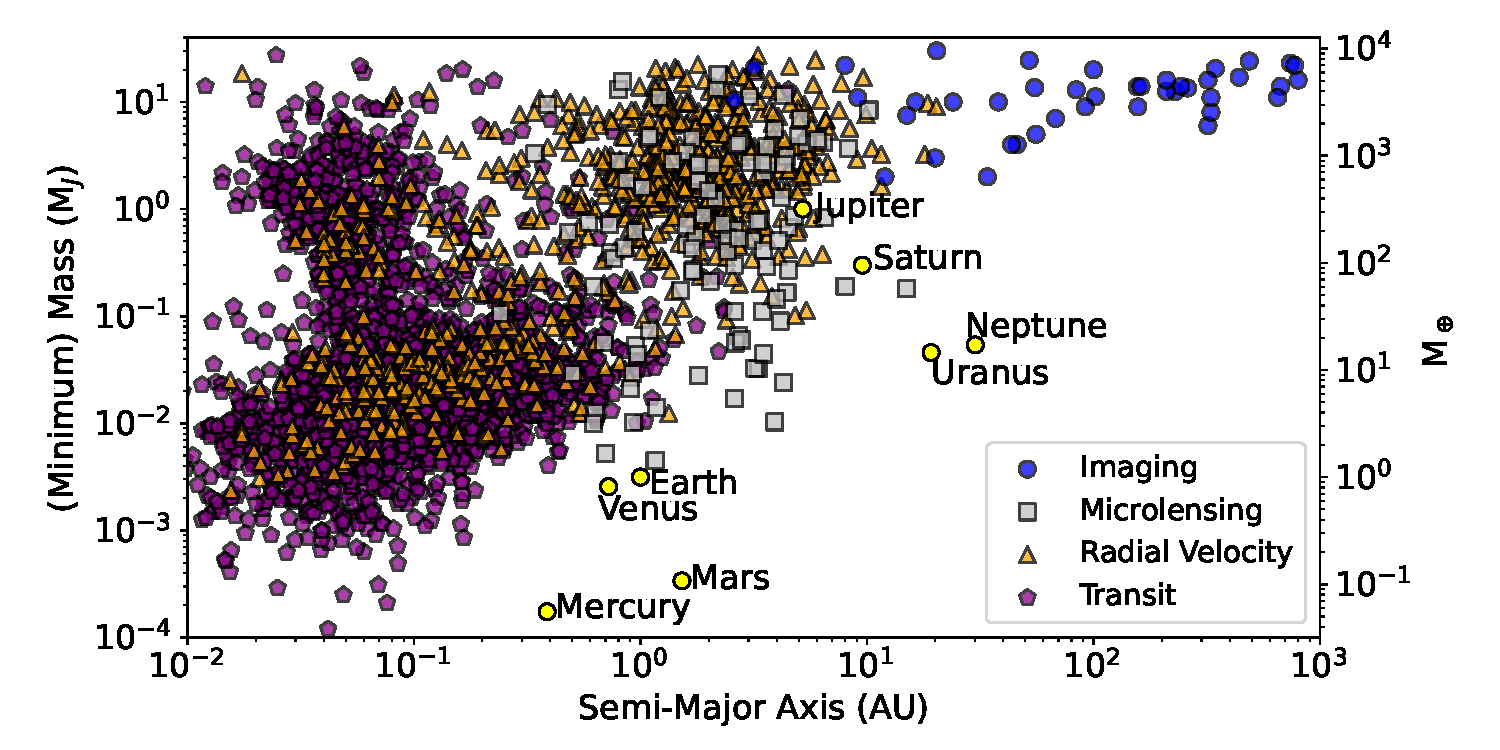
\includegraphics[width=14cm]{figures/all_planets.pdf}
};
}

\frame{
\frametitle{Ways to image more exoplanets}
\tikzoverlay[text width = 14cm] at (0cm, 3cm+4.5pt){
\begin{itemize}
    \item[\textbullet] Improve instruments
    \item[\textbullet] Use the limited observation time more effectively
\end{itemize}
};
\tikzoverlay[text width = 3cm] at (4.5cm-3pt, 1.5cm+4.5pt){
    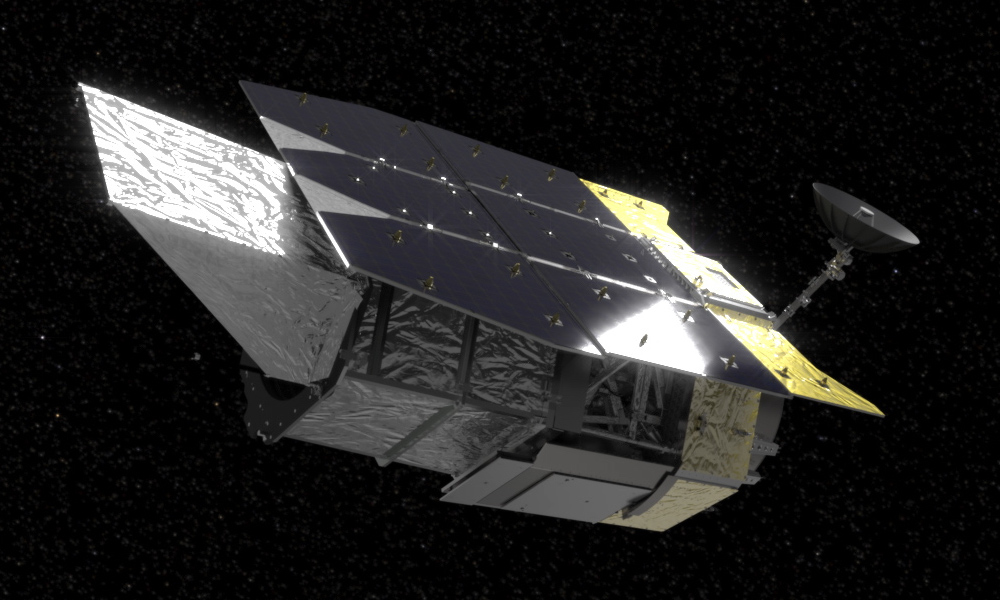
\includegraphics[height=3cm]{figures/roman_space_telescope.jpg}
};
\tikzoverlay[text width = 10cm] at (2cm-7pt, -1.5cm+4.5pt){
    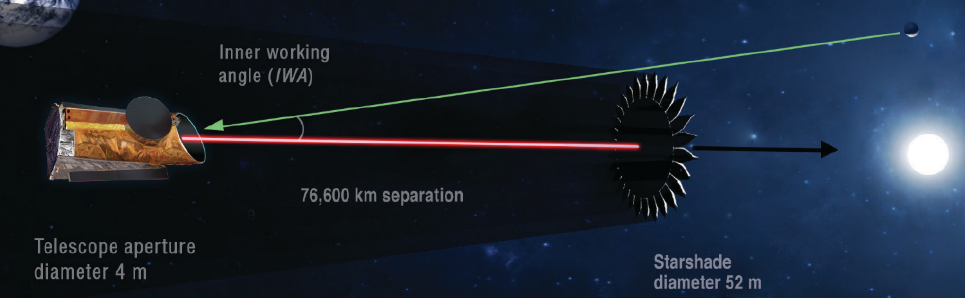
\includegraphics[width=10cm]{figures/habex.png}
};
}

%%%%%%%%%%%%%%%%%%%%%%%%%%%%%%%%%%%%%%%%%%%%%%%%%%%%%%%%%%%%%%%%%%%%%%%%%%%%%%%%%%%%%%%%%%%%%
\section{Radial velocity}
\subsection{Radial velocity} %note that you need both sections and subsection for the navigation to look good for this 
\frame{
    \frametitle{Precursor radial velocity detections}
%\tikzoverlay[text width = 14cm] at (0cm, 3cm+4.5pt){
%\begin{itemize}
    %\item[\textbullet] Detect planets ahead of time via the radial velocity method
    %\item[\textbullet] Currently being used by the Nancy Grace Roman Space Telescope team to identify exoplanet targets
    %\item[\textbullet] The HabEx team notes ``Precise precursor radial velocities (PRVs) will
        %provide multiple advantageous contributions to the scientific yield and optimization of
        %HabEx.''\parencite{HabEx2020}
%\end{itemize}
%};
\tikzoverlay[text width = 14cm] at (0cm, 2.2cm+4.5pt){
    \animategraphics[controls, width=14cm]{10}{rv_example/frame-}{0}{99}
};
}


\frame{
    \frametitle{Radial velocity error}
%\tikzoverlay[text width = 14cm] at (0cm, 3cm+4.5pt){
%\begin{itemize}
    %%\item[\textbullet] Need approximately 10 cm/s precision to detect Earth-like planets
    %\item[\textbullet] For orbit fitting usually given as 1$\sigma $ error in m/s
    %\item[\textbullet] Many sources of error, primarily stellar variability
%\end{itemize}
%};
\tikzoverlay[text width = 6cm] at (0cm-4.5pt, 2cm+4.5pt){
    \animategraphics[controls, width=14cm]{20}{error_example/frame-}{0}{99}
};
%\tikzoverlay[text width = 6cm] at (9.2cm, .5cm+4.9pt){
    %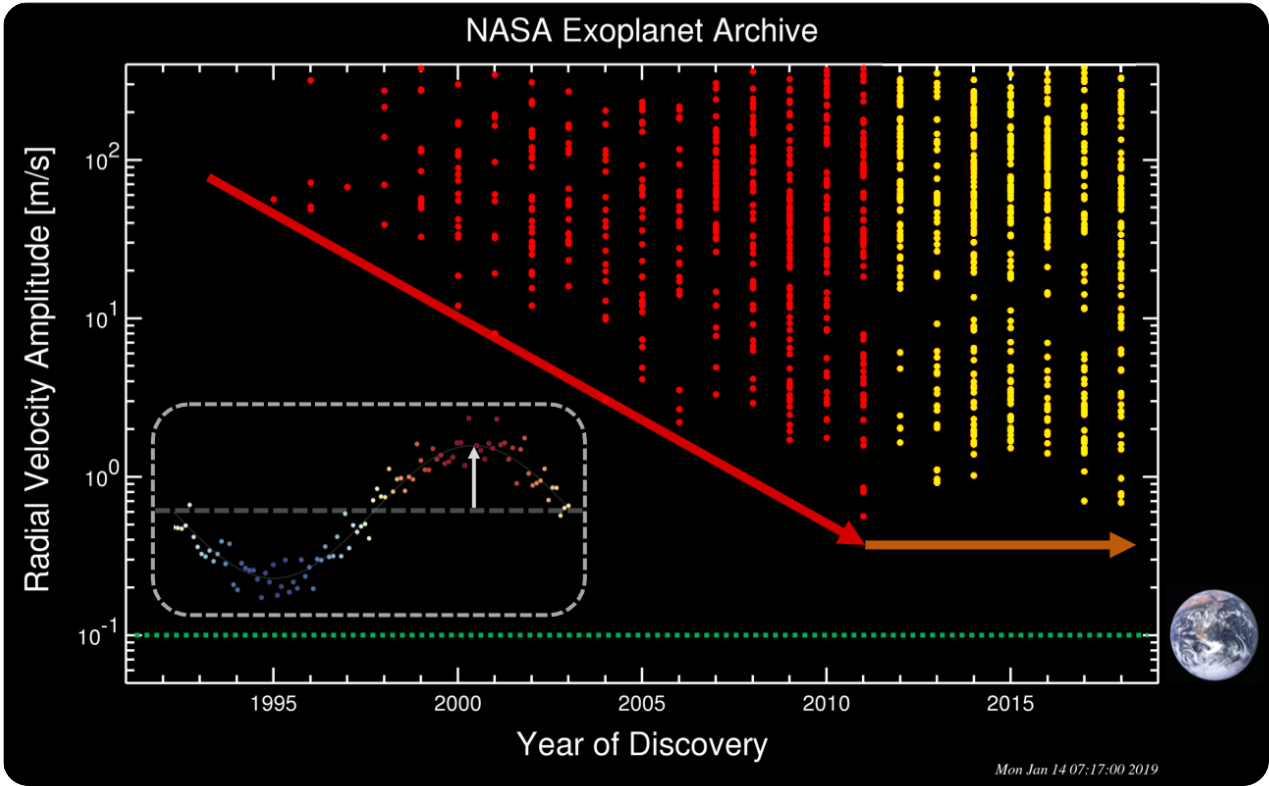
\includegraphics[width=5.5cm]{figures/RV_precision.png}
%};
\footlineextra{\textcite{EPRV2020} }
}

\frame{
    \frametitle{Mass/inclination ambiguity}
\tikzoverlay[text width = 6cm] at (1cm, 3cm+4.5pt){
    \animategraphics[loop, controls, width=12cm]{10}{mass_inclination_comparision/frame-}{0}{99}
};
}

%%%%%%%%%%%%%%%%%%%%%%%%%%%%%%%%%%%%%%%%%%%%%%%%%%%%%%%%%%%%%%%%%%%%%%%%%%%%%%%%%%%%%%%%%%%%%
\section{Direct imaging}
\subsection{Direct imaging}

\frame{
    \frametitle{Geometric constraint}
\tikzoverlay[text width = 6cm] at (-1cm, 3cm+4.5pt){
    \animategraphics[loop, controls, width=12cm]{10}{geometric_detection_criteria/frame-}{0}{99}
};
\tikzoverlay[text width = 3cm] at (11cm, 1cm+4.5pt){
    \center{distance = $d$}
    \begin{align*}
        \alpha = \tan^{-1}\left( \frac{s}{d} \right)
    \end{align*}
    \begin{align*}
        \boxed{\textrm{IWA} < \alpha < \textrm{OWA}}
    \end{align*}
};
}
\frame{
    \frametitle{Photometric constraint}
\tikzoverlay[text width = 6cm] at (-1cm, 3cm+4.5pt){
    \animategraphics[loop, controls, width=12cm]{10}{photometric_detection_criteria/frame-}{0}{99}
};
\tikzoverlay[text width = 3cm] at (11cm, 1.5cm+4.5pt){
    \begin{align*}
        F_R = \frac{F_p}{F_s}
    \end{align*}
    \begin{align*}
        \Delta \textrm{mag} = -2.5 \log_{10}F_R
    \end{align*}

    \begin{align*}
            \boxed{\Delta \textrm{mag} < \Delta \textrm{mag}_0}
    \end{align*}
};
}


\frame{
    \frametitle{Both constraints}
\tikzoverlay[text width = 6cm] at (1cm, 3cm+4.5pt){
    \animategraphics[loop, controls, width=12cm]{10}{both_detection_criteria/frame-}{0}{99}
};
}


%%%%%%%%%%%%%%%%%%%%%%%%%%%%%%%%%%%%%%%%%%%%%%%%%%%%%%%%%%%%%%%%%%%%%%%%%%%%%%%%%%%%%%%%%%%%%
\section{Predicting detectability}
\subsection{Predicting detectability}
\frame{
    \frametitle{Questions about using RV data for imaging}
\tikzoverlay[text width = 14cm] at (0cm, 2.5cm+4.5pt){
\begin{itemize}
    \item[\textbullet] How should we use the incomplete RV information to predict when a planet is detectable?
    \item[\textbullet] How long is RV data useful for scheduling direct imaging observations?
\end{itemize}
};
}
%\frame{
%\frametitle{Completeness, $C$}
%\tikzoverlay[text width = 6cm] at (0cm, 2.5cm+4.5pt){
%\begin{enumerate}
    %\item[\textbullet] Simulation based metric that calculates the probability of detecting a planet around a target
        %star, should a planet in the assumed population exist
    %\item[\textbullet] With enough simulated planets $C$ is constant
    %\item[\textbullet] Useful when there are no prior detections around a star
%\end{enumerate}
%\begin{align*}
    %C = \frac{\textrm{\# of detectable simulated planets}}{\textrm{\# of simulated planets}}
%\end{align*}
%};
%\tikzoverlay[text width = 7cm] at (7cm, 3.1cm+4.5pt){
    %\animategraphics[loop, controls, width=7cm]{10}{completeness/frame-}{0}{99}
%};
%\footlineextra{\textcite{Brown2004c}, \textcite{Brown2005d}, \textcite{Garrett2016}}
%}
%\frame{
%\frametitle{Completeness, $C$}
%\tikzoverlay[text width = 12cm] at (0cm, 3.1cm+4.5pt){
    %\animategraphics[loop, controls, width=14cm]{10}{comp_constraint/frame-}{0}{99}
%};
%}

\frame{
\frametitle{Probability of detection, $P_{\textrm{det}}$}
\tikzoverlay[text width = 14cm] at (0cm, 3cm+4.5pt){
\begin{itemize}
    \item[\textbullet] Probability that the planet that created the RV signal is detectable at a
        time
    \item[\textbullet] Calculate it by constructing orbits that are consistent with the RV signal
        and compute $P_{\textrm{det}}(t)$ over necessary times
\end{itemize}
\begin{align*}
    P_{\textrm{det}}(t) = \frac{\textrm{\# of constructed orbits detectable at time $t$}}{\textrm{\# of constructed orbits}}
\end{align*}
};
}
\frame{
\frametitle{Probability of detection: simple example}
\tikzoverlay[text width = 14cm] at (0cm, 3.5cm+4.5pt){
\begin{align*}
    P_{\textrm{det}}(t) = \frac{\textrm{\# of constructed orbits detectable at time $t$}}{\textrm{\# of constructed orbits}}
\end{align*}
};
\tikzoverlay[text width = 7cm] at (0cm-3pt, 2.2cm+4.5pt){
    \animategraphics[controls, width=14cm]{10}{pdet/frame-}{0}{99}
};
}

\frame{
\frametitle{What needs to be studied about $P_{\textrm{det}}$}
\tikzoverlay[text width = 14cm] at (0cm, 3.1cm+4.5pt){
\begin{itemize}
    \item[\textbullet] The best way to ``construct orbits''
    \item[\textbullet] The limitations and potential failures of predicting detectability from RV
        fits
\end{itemize}
};
}

%%%%%%%%%%%%%%%%%%%%%%%%%%%%%%%%%%%%%%%%%%%%%%%%%%%%%%%%%%%%%%%%%%%%%%%%%%%%%%%%%%%%%%%%%%%%%
\section{Constructing orbits}%
\subsection{Constructing orbits}
\frame{
\frametitle{Initial work}
\tikzoverlay[text width = 14cm] at (0cm, 3.2cm+4.5pt){
\begin{enumerate}
    \item[\textbullet] Assumption that RV orbit fits would grow worse in time
    \item[\textbullet] HabEx report notes that fits go ``stale'' and recommends RV measurements ``up
        until, during, and after mission launch'' \parencite{HabEx2020}
    \item[\textbullet] Simple study that sampled orbital elements independently
\end{enumerate}
};
\tikzoverlay[text width = 14cm] at (3cm-4.5pt, .85cm+4.5pt){
    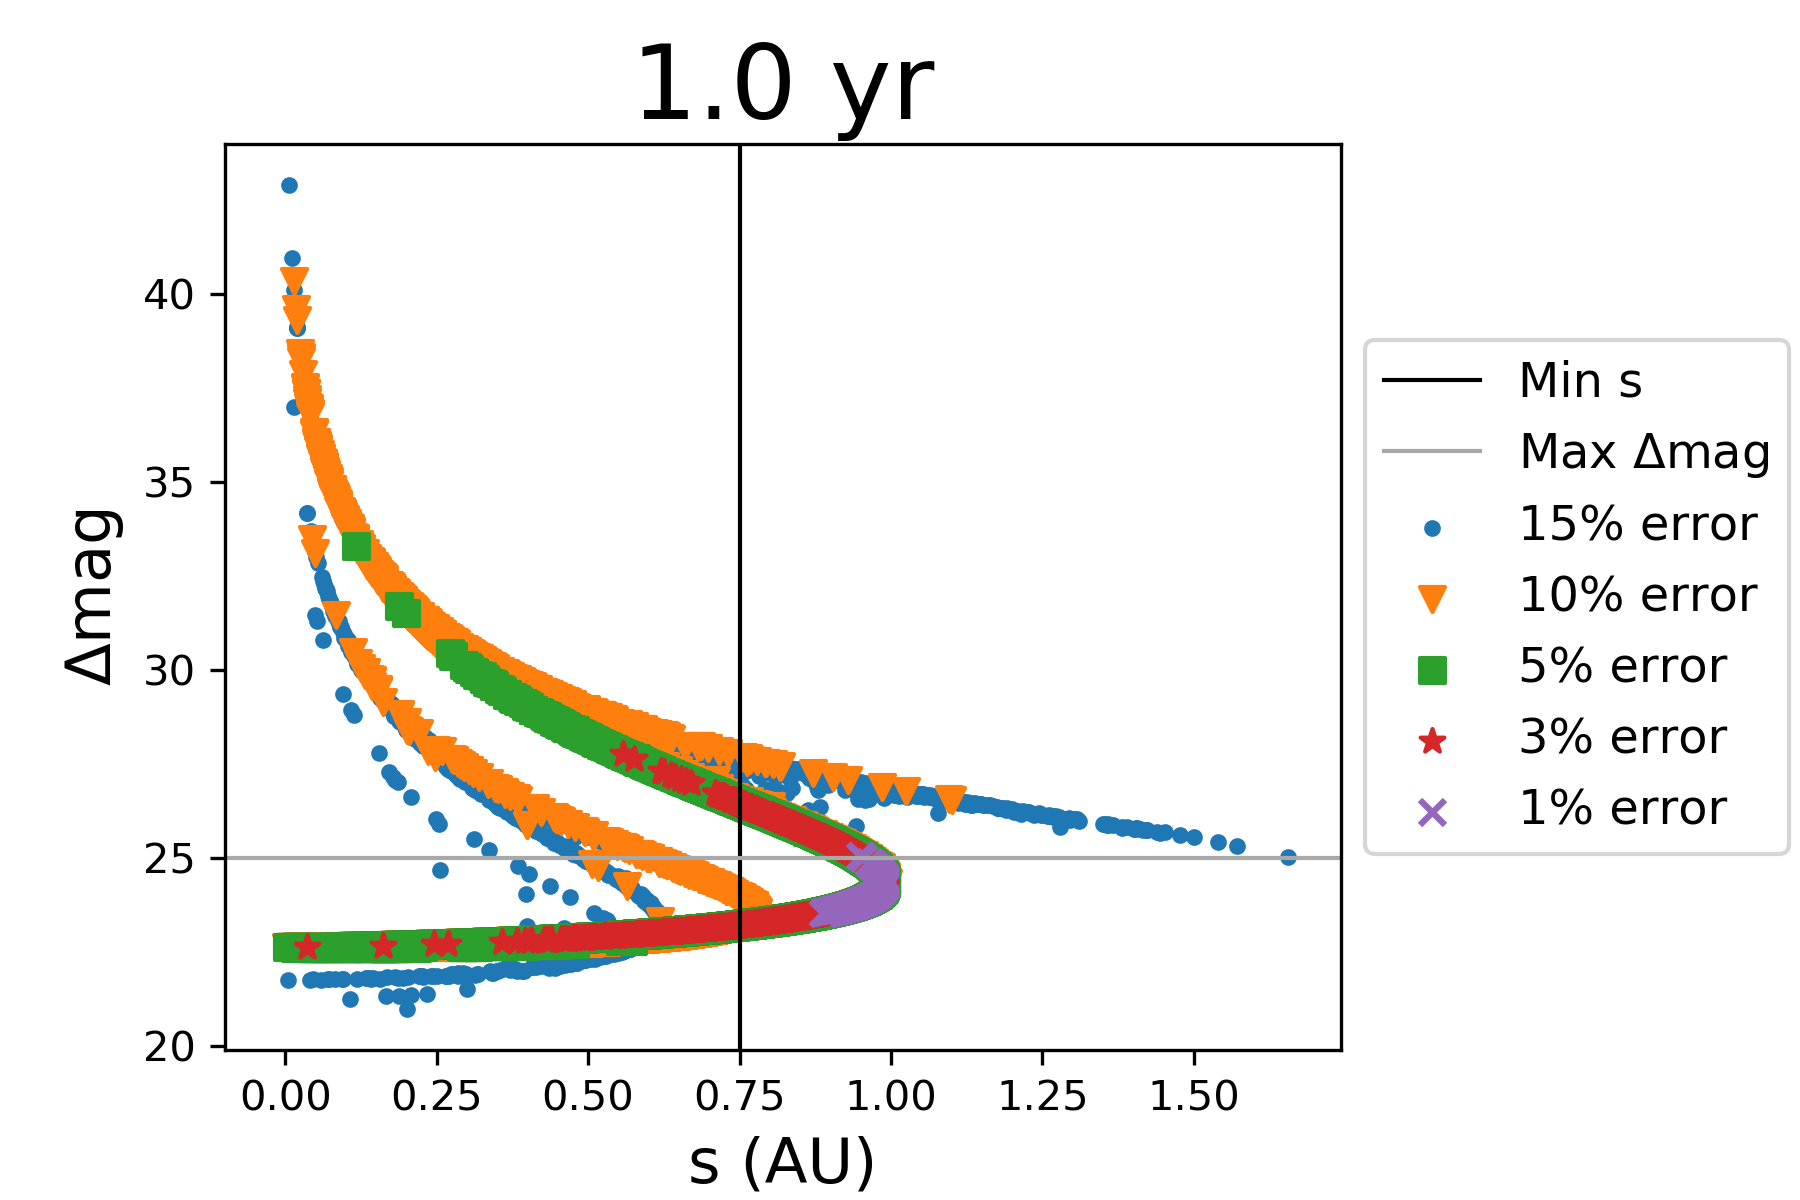
\includegraphics[width=8cm]{figures/initial_work.png}
};
}
\frame{
\frametitle{Fitting RV curves}
\tikzoverlay[text width = 14cm] at (0cm, 3cm+4.5pt){
\begin{enumerate}
    \item[\textbullet] Want to start with RV data instead of sampling orbital elements directly
    %\item[\textbullet] Lots of study and techniques already to fit orbits to RV
    \item[\textbullet] Use the industry standard RadVel\parencite{Fulton2018}, a Bayesian RV orbit fitting tool
\end{enumerate}
};
\tikzoverlay[text width = 1cm] at (-.5cm-4.5pt, 0cm+4.5pt){
    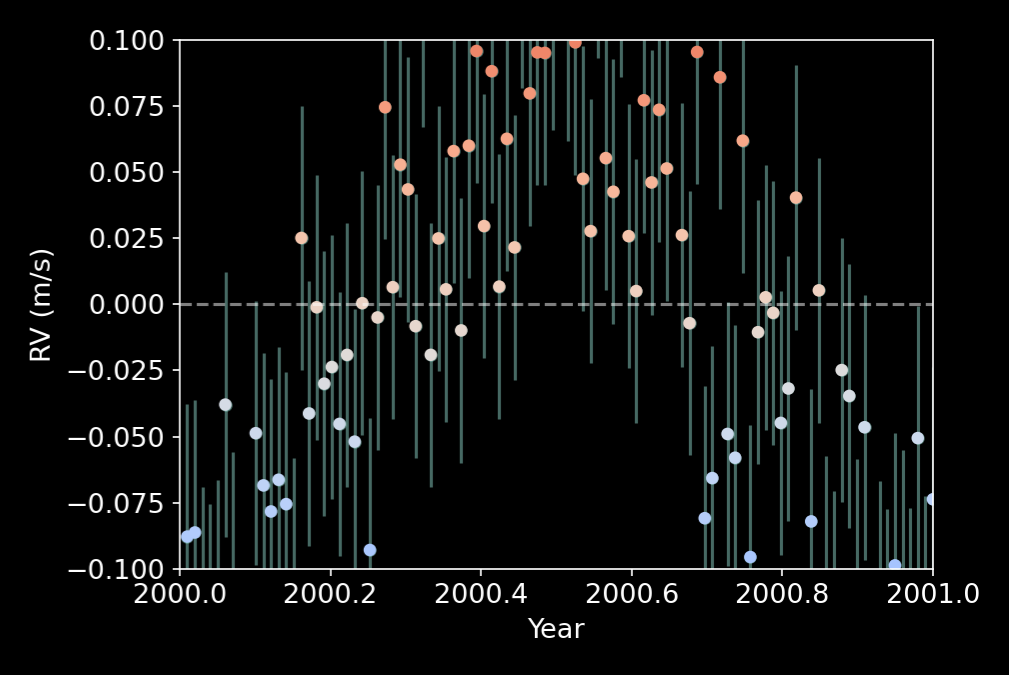
\includegraphics[width=5cm]{figures/simple_rv_curve.png}
};
\tikzoverlay[text width = 1cm] at (5.5cm-4.5pt, -.6cm+4.5pt){
    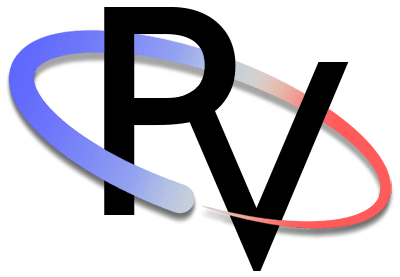
\includegraphics[width=3cm]{figures/radvel_logo_alpha_retina.png}
};
\tikzoverlay[text width = 5cm] at (9cm-4.5pt, 0.51cm+4.5pt){
    Fitted orbital elements
    \begin{itemize}
        \item Orbital period, $T$
        \item Eccentricity, $e$
        \item Argument of periapsis, $\omega$
        \item Time of conjunction, $T_c$
        \item RV semi-amplitude,  $K$
    \end{itemize}
};
\tikzoverlay[text width = 1cm] at (8.66, .16){
\begin{tikzpicture}[ultra thick]
    \draw[decorate, decoration ={brace}] (0, 0) -- (0, 2.75);
\end{tikzpicture}
};
\tikzoverlay[text width = 2cm] at (4cm, -1.2cm){
\begin{tikzpicture}[ultra thick]
    \draw [-to] (1, 2) -- (2, 2);
    \draw [-to] (4.5, 2) -- (5.5, 2);
\end{tikzpicture}
};

}

\frame{
\frametitle{RadVel output}
%\tikzoverlay[text width = 14cm] at (0cm, 3cm+4.5pt){
%%\begin{enumerate}
    %\item[\textbullet] RadVel provides every set of orbital elements it tests while fitting the RV
        %data and an associated probability for every set of elements
%\end{enumerate}
%};
\tikzoverlay[text width=10cm] at (2cm, 2.3cm){
\begin{table}[htpb]
\begin{adjustbox}{max width=1\textwidth}
    \centering
    \begin{tabular}{|c|c|c|c|c|}
        \hline
        \textbf{Step} & \textbf{0} & \textbf{1} & \textbf{\ldots} & \textbf{224999} \\
        \hline
        $T$ (d) & 671.93 & 671.81 & \ldots & 672.86 \\
        $T_c$ (jd) & 2452269.85 & 2452270.68 & \ldots & 2452268.53 \\
        $\sqrt{e} \cos{\omega_s }$ & 0.090 & 0.072 & \ldots & 0.090 \\
        $\sqrt{e} \sin{\omega_s} $ & -0.049 & -0.044 & \ldots & 0.019 \\
        $K$ (m/s) & 0.996 & 0.995 & \ldots & 1.00\\
        $\ln\left( \textrm{Probability} \right)$& 8.15 & 8.32 & \ldots & 4.07\\
        \hline
    \end{tabular}
    %\label{tab:radvel_output}
\end{adjustbox}
    %\caption{RadVel output}
\end{table}
};
%\tikzoverlay[text width = 14cm] at (0cm, -2.5cm+4.5pt){
%\begin{enumerate}
    %\item[\textbullet] To calculate $P_{\textrm{det}}$ we have to be able to propagate in time
    %\item[\textbullet] Need process to go from RadVel output to all necessary orbital elements
%\end{enumerate}
%};
}

\frame{
    \frametitle{Converting RadVel outputs}
\tikzoverlay[text width = 14cm] at (0cm, 3.3cm+4.5pt){
\begin{enumerate}
    \item[\textbullet] To calculate $P_{\textrm{det}}$ we need more than just what RadVel provides
        since we need to propagate the orbits in time
    %\item[\textbullet] Solve for some orbital elements with standard orbital mechanics
\end{enumerate}
};
\tikzoverlay[text width=10cm] at (2cm, 2.0cm){
\begin{table}[h!]
    \begin{adjustbox}{max width=1\textwidth}
    \begin{tabular}{|l|l|l|}
        \hline
        Element & From RadVel & Equations \\
        \hline
        $a$ & $T$ & $a = \left( G M_s \left( \frac{T}{2 \pi } \right) \right)^{\frac{1}{3}}$ \\
        \hline
         $e$ & $\sqrt{e} \cos{\omega_s}$, $\sqrt{e} \sin{\omega_s}$ & $e = \left( \sqrt{e} \cos{\omega_s} \right)^2 + \left( \sqrt{e} \sin{\omega_s} \right)^2$ \\
        \hline
        $\omega_p$ & $\sqrt{e} \cos{\omega_s}$, $\sqrt{e} \sin{\omega_s}$ & $\omega_s = \arctan\left( \frac{\sqrt{e} \sin{\omega_s}}{\sqrt{e} \cos{\omega_s}} \right) $ \\
         & & $\omega_p = \omega_s + \pi $\\
         \hline
        $T_p$ & $T$, $e$, $\omega_s$, $T_c$ & $\nu_p = \frac{\pi}{2} - \omega_s$ \\
          & & $\tan\left( \frac{E}{2} \right) = \sqrt{\frac{1-e}{1+e}} \tan\left( \frac{\nu}{2} \right) $ \\
          & & $M = E - e \sin E$ \\
          & & $T_p = T_c - \frac{M T}{2 \pi }$ \\
        \hline
        $M_p \sin i$ & $K$, $T$, $e$ & $M_p \sin i = \left( \frac{T}{2 \pi G} \right)^{\frac{1}{3}} K M_s^{\frac{2}{3}} \sqrt{1 -e^2} $\\
        \hline
\end{tabular}
\end{adjustbox}
%\caption{Orbital element equations}
\end{table}
};
}

\frame{
    \frametitle{Resolving mass/inclination ambiguity}
\tikzoverlay[text width = 14cm] at (0cm, 3cm+4.5pt){
\begin{itemize}
    \item[\textbullet] Have everything necessary for propagation except inclination
    \item[\textbullet] Assume that inclinations are distributed isotropically in the universe, which
        creates a sinusoidal distribution in $[0, \pi)$ \parencite{Savransky2011a}
    %\item[\textbullet] Remove inclinations that would result in hydrogen burning mass ($0.08
        %M_{\odot}$ )
\end{itemize}
};
\tikzoverlay[text width = 5cm] at (-1.1cm, 0.85cm){
    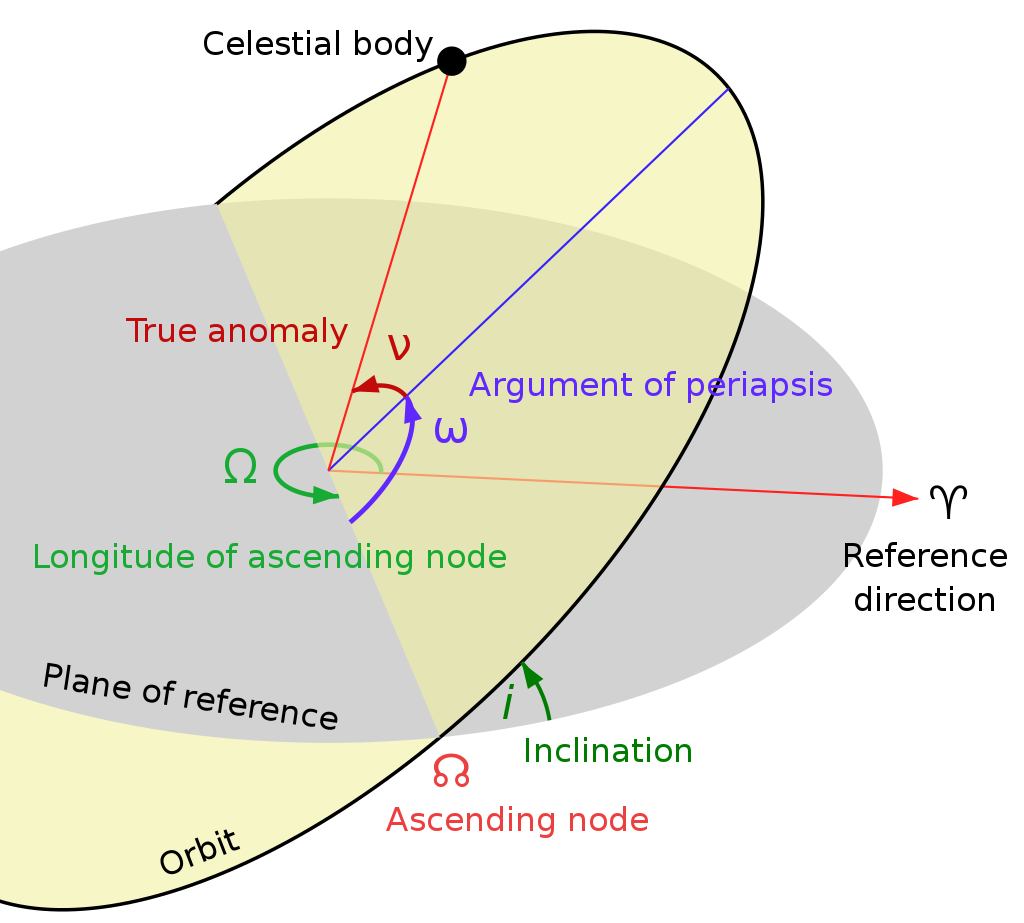
\includegraphics[width=5cm]{orbelem.png}
};
\tikzoverlay[text width = 5cm] at (3.75cm, 0.80cm){
    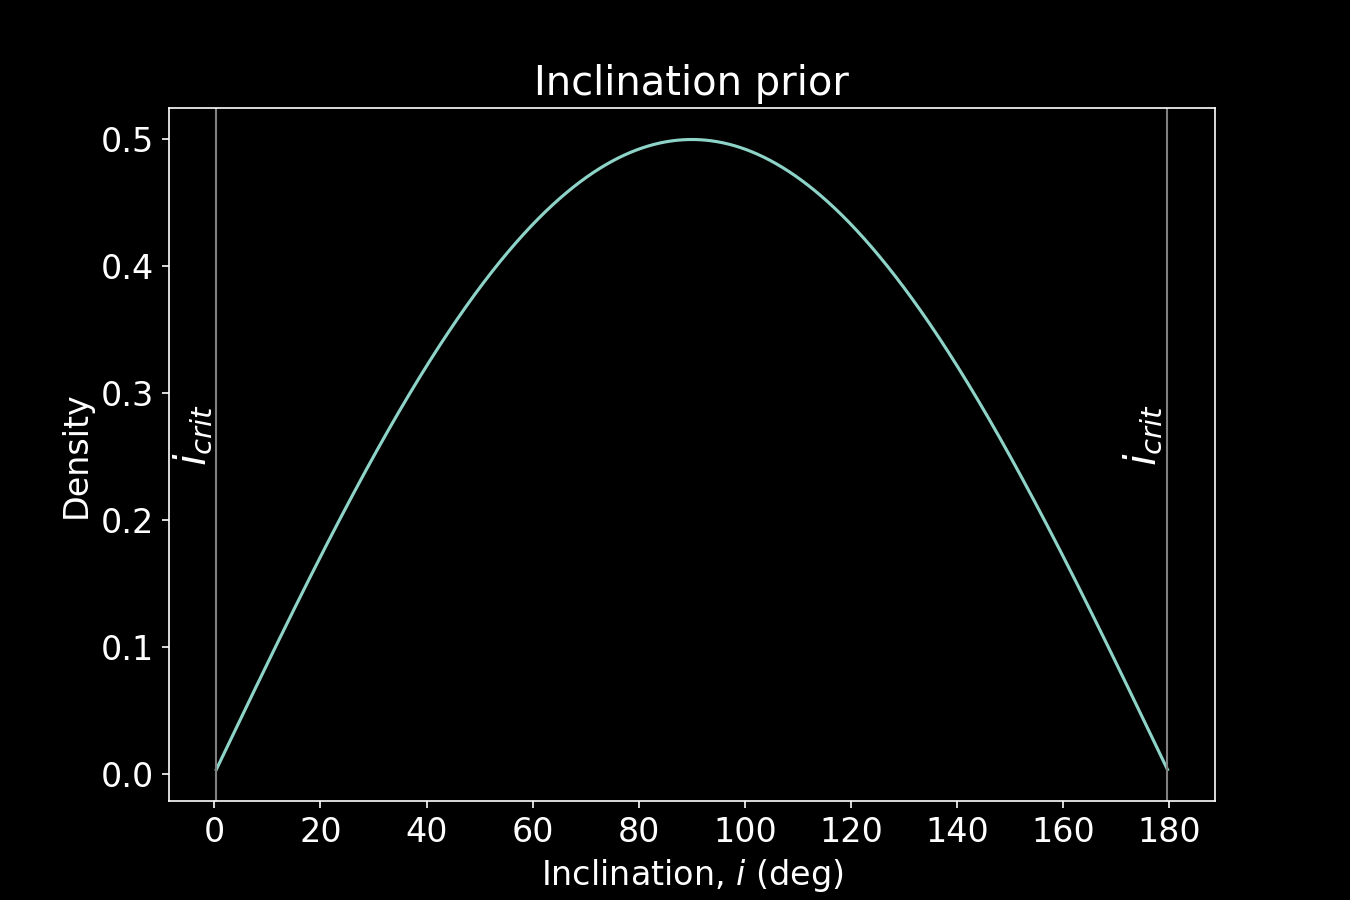
\includegraphics[width=7cm]{inc_distribution.png}
};
\tikzoverlay[text width = 5cm] at (10.15cm, -0.6cm){
    \begin{align*}
        i_{\textrm{crit}} = \sin^{-1}\left( \frac{M_p \sin i}{0.08 M_{\odot}} \right) 
    \end{align*}
};
\footlineextra{Wikipedia}
}

\frame{
    \frametitle{Calculating planet radius}
%\tikzoverlay[text width = 14cm] at (0cm, 3cm+4.5pt){
%\begin{itemize}
    %\item[\textbullet] Use a mass-radius relationship to calculate planet radius from mass
%\end{itemize}
%};
\tikzoverlay[text width = 5cm] at (2cm, 3.1cm){
    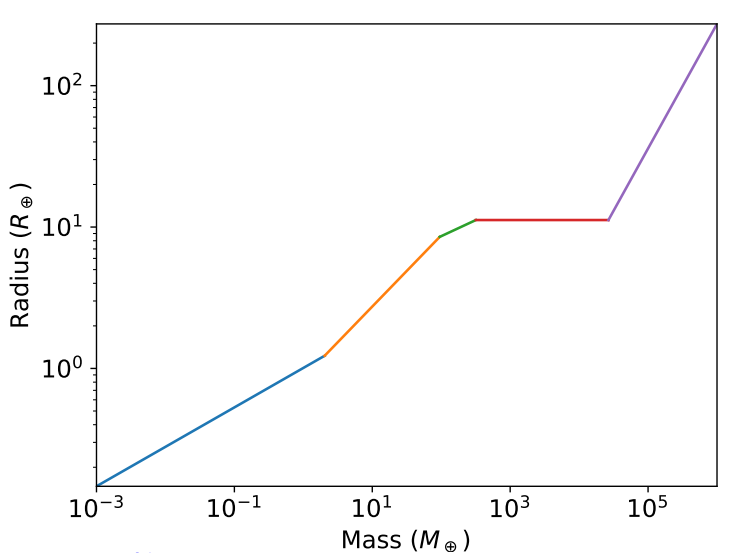
\includegraphics[width=9cm]{ForecasterMod.png}
};
\footlineextra{\textcite{Savransky2019SPIE}, \textcite{Forecaster}}
}

\frame{
\frametitle{Construction methods}
\tikzoverlay[text width = 14cm] at (0cm, 3cm+4.5pt){
    \begin{itemize}
        \item[\textbullet] For $P_{\textrm{det}}$ we need thousands of orbits
        \item[\textbullet] General outline for constructing orbits 
        \begin{enumerate}
            \item[1)] Generate 50,000 sets of fitting basis parameters based on RadVel output
            \item[2)] Convert the fitting basis parameter sets into standard orbital elements
            \item[3)] Sample 50,000 inclinations to resolve $M_p \sin{i}$ ambiguity for each set of
                orbital elements
        \end{enumerate}
        \item[\textbullet] Studied four methods of generating the 50,000 sets of fitting basis
            parameters, called ``construction methods''
        \begin{enumerate}
            \item[1)] Max likelihood
            \item[2)] Max kernel density estimate (KDE)
            \item[3)] Credible interval
            \item[4)] Multivariate Gaussian
        \end{enumerate}
    \end{itemize}
};
}

\frame{
\frametitle{Method 1: max likelihood}
%\tikzoverlay[text width = 14cm] at (0cm, 3cm+4.5pt){
    %\begin{itemize}
        %\item[\textbullet] Generated by the RadVel reports and often referenced
        %\item[\textbullet] Choose RadVel step with the highest reported $\ln \left(\textrm{Probability}\right)$
        %\item[\textbullet] Use the same fitting basis set ($T$, $T_c$, $e$, $\omega_s$, $K$) 50,000 times
            %\hrule
    %\end{itemize}
%};
\tikzoverlay[text width=10cm] at (2cm, 2cm){
\begin{table}[htpb]
\begin{adjustbox}{max width=1\textwidth}
    \centering
    \begin{tabular}{|c|c|c|c|c|}
        \hline
        \textbf{Step} & \textbf{0} &  \textbf{1} & \textbf{\ldots} & \textbf{224999} \\
        \hline
        $T$ (d) & 671.93 & \cellcolor[rgb]{0,1,0} 671.81 & \ldots & 672.86 \\
        $T_c$ (jd) & 2452269.85 & \cellcolor[rgb]{0,1,0} 2452270.68 & \ldots & 2452268.53 \\
        $\sqrt{e} \cos{\omega_s }$ & 0.090 & \cellcolor[rgb]{0,1,0} 0.072 & \ldots & 0.090 \\
        $\sqrt{e} \sin{\omega_s} $ & -0.049 & \cellcolor[rgb]{0,1,0} -0.044 & \ldots & 0.019 \\
        $K$ (m/s) & 0.996 & \cellcolor[rgb]{0,1,0} 0.995 & \ldots & 1.00\\
        $\ln\left( \textrm{Probability} \right)$& 8.15 & \cellcolor[rgb]{0,1,0} 8.32 & \ldots & 4.07\\
        \hline
    \end{tabular}
    %\label{tab:radvel_output}
\end{adjustbox}
    %\caption{RadVel output}
\end{table}
};
\tikzoverlay[text width = 1cm] at (6.5cm, 3.3cm){
\begin{tikzpicture}[ultra thick]
    \draw[decorate, decoration ={brace}] (1.5cm, -2cm) -- node[above=0.2cm and 0cm]{x 50,000} (4cm,
        -2cm);
    %\draw[-to] (7cm, -1cm) -- node[above left=0.2cm and -2.2cm]{Maximize KDE} (10cm, -2cm);
\end{tikzpicture}
};
}
\frame{
    \frametitle{Method 1: max likelihood visualization}
\tikzoverlay[text width = 10cm] at (0cm-3pt, 3.1cm+4.5pt){
    \animategraphics[loop, controls, width=14cm]{20}{ML_vis/frame-}{0}{99}
};
}

\frame{
\frametitle{Method 2: max KDE}
%\tikzoverlay[text width = 14cm] at (0cm, 3cm+4.5pt){
    %\begin{itemize}
        %\item[\textbullet] Create kernel density estimate (KDE) based on every step, then calculate
            %the fitting basis set that maximizes the KDE
        %\item[\textbullet] Use the same fitting basis set ($T$, $T_c$, $e$, $\omega_s$, $K$) 50,000 times
            %\hrule
    %\end{itemize}
%};
\tikzoverlay[text width=10cm] at (-.3cm, 1cm){
    \definecolor{kde}{gray}{0.7}
\begin{table}[htpb]
\begin{adjustbox}{max width=1\textwidth}
    \centering
    \begin{tabular}{|c|c|c|c|c|}
        \hline
        \textbf{Step} & \textbf{0} &  \textbf{1} & \textbf{\ldots} & \textbf{224999} \\
        \hline
        $T$ (d) &\cellcolor{kde} 671.93 &\cellcolor{kde} \cellcolor{kde} 671.81 &\cellcolor{kde} \ldots &\cellcolor{kde} 672.86 \\
        $T_c$ (jd) &\cellcolor{kde} 2452269.85 &\cellcolor{kde} \cellcolor{kde} 2452270.68 &\cellcolor{kde} \ldots &\cellcolor{kde} 2452268.53 \\
        $\sqrt{e} \cos{\omega_s }$ &\cellcolor{kde} 0.090 &\cellcolor{kde} \cellcolor{kde} 0.072 &\cellcolor{kde} \ldots &\cellcolor{kde} 0.090 \\
        $\sqrt{e} \sin{\omega_s} $ &\cellcolor{kde} -0.049 &\cellcolor{kde} \cellcolor{kde} -0.044 &\cellcolor{kde} \ldots &\cellcolor{kde} 0.019 \\
        $K$ (m/s) &\cellcolor{kde} 0.996 & \cellcolor{kde} 0.995 &\cellcolor{kde} \ldots &\cellcolor{kde} 1.00\\
        $\ln\left( \textrm{Probability} \right)$& 8.15 &  8.32 & \ldots & 4.07\\
        \hline
    \end{tabular}
    %\label{tab:radvel_output}
\end{adjustbox}
    %\caption{RadVel output}
\end{table}
};
\tikzoverlay[text width = 1cm] at (2.1cm, 2cm){
\begin{tikzpicture}[ultra thick]
    \draw[decorate, decoration ={brace}] (0, -1.5) -- node[above left=6pt and -2cm]{Calculate
        KDE with} (7.5, -1.5);
    %\draw[-to] (7cm, -1cm) -- node[above left=0.2cm and -2.2cm]{Maximize KDE} (10cm, -2cm);
\end{tikzpicture}
};
\tikzoverlay[text width = 5cm] at (9.5cm, 0cm){
\begin{center}
Maximize KDE to get set of
\linebreak
($T$, $T_c$, $e$, $\omega_s$, $K$)
\linebreak
then use it 50,000 times
\end{center}
};
}

\frame{
    \frametitle{Method 2: max KDE visualization}
\tikzoverlay[text width = 10cm] at (0cm-3pt, 3.1cm+4.5pt){
    \animategraphics[loop, controls, width=14cm]{20}{MKDE_vis/frame-}{0}{99}
};
}

\frame{
\frametitle{Method 3: credible interval}
%\tikzoverlay[text width = 14cm] at (0cm, 3cm+4.5pt){
    %\begin{itemize}
        %\item[\textbullet] For each element in the basis ($T$, $T_c$, $e$, $\omega_s$, $K$)
            %calculate the median and standard deviation over all of the steps
        %\item[\textbullet] Sample each element as a normal distribution 50,000 times
            %\hrule
    %\end{itemize}
%};
    \definecolor{t}{gray}{0.9}
    \definecolor{tc}{gray}{0.85}
    \definecolor{ce}{gray}{0.8}
    \definecolor{se}{gray}{0.75}
    \definecolor{k}{gray}{0.7}
    \tikzoverlay[text width=10cm] at (-.3cm, 1cm){
    \begin{table}[htpb]
    \begin{adjustbox}{max width=1\textwidth}
        \centering
        \begin{tabular}{|c|c|c|c|c|}
            \hline
            \textbf{Step} & \textbf{0} & \textbf{1} &\textbf{\ldots} &\textbf{224999} \\
            \hline
            $T$ (d) &\cellcolor{t} 671.93 &\cellcolor{t} \cellcolor{t} 671.81 &\cellcolor{t} \ldots &\cellcolor{t} 672.86 \\
            $T_c$ (jd) &\cellcolor{tc} 2452269.85 &\cellcolor{tc} \cellcolor{tc} 2452270.68 &\cellcolor{tc} \ldots &\cellcolor{tc} 2452268.53 \\
            $\sqrt{e} \cos{\omega_s }$ &\cellcolor{ce} 0.090 &\cellcolor{ce} \cellcolor{ce} 0.072 &\cellcolor{ce} \ldots &\cellcolor{ce} 0.090 \\
            $\sqrt{e} \sin{\omega_s} $ &\cellcolor{se} -0.049 &\cellcolor{se} \cellcolor{se} -0.044 &\cellcolor{se} \ldots &\cellcolor{se} 0.019 \\
            $K$ (m/s) &\cellcolor{k} 0.996 & \cellcolor{k} 0.995 &\cellcolor{k} \ldots &\cellcolor{k} 1.00\\
            $\ln\left( \textrm{Probability} \right)$& 8.15 & 8.32 & \ldots & 4.07\\
            \hline
        \end{tabular}
        %\label{tab:radvel_output}
    \end{adjustbox}
        %\caption{RadVel output}
    \end{table}
};
    \tikzoverlay[text width = 5cm] at (9.6, 1cm){
    \begin{tikzpicture}[ultra thick]
        \draw[decorate, decoration ={brace}, color=t] (2.5cm, -1.25cm) -- node[left=1cm and -1cm]{} (2.5cm,
            -1.7cm);
        \draw[decorate, decoration ={brace}, color=tc] (2.5cm, -1.7cm) -- node[left=1cm and -1cm]{} (2.5cm,
            -2.1cm);
        \draw[decorate, decoration ={brace}, color=ce] (2.5cm, -2.1cm) -- node[left=1cm and -1cm]{} (2.5cm,
            -2.55cm);
        \draw[decorate, decoration ={brace}, color=se] (2.5cm, -2.55cm) -- node[left=1cm and -1cm]{} (2.5cm,
            -2.95cm);
        \draw[decorate, decoration ={brace}, color=k] (2.5cm, -2.95cm) -- node[left=1cm and -1cm]{} (2.5cm,
            -3.4cm);
        %\draw[-to] (7cm, -1cm) -- node[above left=0.2cm and -2.2cm]{Maximize KDE} (10cm, -2cm);
    \end{tikzpicture}
};
    \tikzoverlay[text width = 3cm] at (10cm, -0.5cm){
    Sample normal distributions for each parameter 50,000 times
};
%\tikzoverlay[text width = 5cm] at (9.5cm, -1cm){
%\begin{center}
%Maximize KDE to get set of
%\linebreak
%($T$, $T_c$, $e$, $\omega_s$, $K$)
%\linebreak
%then use it 50,000 times
%\end{center}
%};
}
\frame{
    \frametitle{Method 3: credible interval visualization}
\tikzoverlay[text width = 10cm] at (0cm-3pt, 3.1cm+4.5pt){
    \animategraphics[loop, controls, width=14cm]{20}{CI_vis/frame-}{0}{99}
};
}

\frame{
    \frametitle{Method 4: multivariate Gaussian}
    %\tikzoverlay[text width = 14cm] at (0cm, 3cm+4.5pt){
        %\begin{itemize}
            %\item[\textbullet] Take 1000 steps with largest probability
            %\item[\textbullet] Calculate covariance matrix between ($T$, $T_c$, $e$, $\omega_s$, $K$) based on those steps
            %\item[\textbullet] Sample multivariate normal distribution 50,000 times to get sets of
                %orbital elements
                %\hrule
        %\end{itemize}
    %};
    \tikzoverlay[text width=10cm] at (-.3cm, 2.5cm){
        \definecolor{mg}{rgb}{0, 1, 0}
    \begin{table}[htpb]
    \begin{adjustbox}{max width=1\textwidth}
        \centering
        \begin{tabular}{|c|c|c|c|c|}
            \hline
            \textbf{Step} & \textbf{0}& \textbf{1} &\textbf{\ldots} &\textbf{224999} \\
            \hline
            $T$ (d) &671.93 \cellcolor{mg}&\cellcolor{mg}671.81 &\ldots &672.86 \\
            $T_c$ (jd) &2452269.85 \cellcolor{mg}&\cellcolor{mg}2452270.68 &\ldots &2452268.53 \\
            $\sqrt{e} \cos{\omega_s }$ &0.090 \cellcolor{mg}&\cellcolor{mg}0.072 &\ldots &0.090 \\
            $\sqrt{e} \sin{\omega_s} $ &-0.049 \cellcolor{mg}&\cellcolor{mg}-0.044 &\ldots &0.019 \\
            $K$ (m/s) &0.996 \cellcolor{mg}&\cellcolor{mg} 0.995 &\ldots &1.00\\
            $\ln\left( \textrm{Probability} \right)$& \cellcolor{mg} 8.15 & \cellcolor{mg}  8.32 & \ldots & 4.07\\
            \hline
        \end{tabular}
        %\label{tab:radvel_output}
    \end{adjustbox}
        %\caption{RadVel output}
    \end{table}
    };
    \tikzoverlay[text width = 1cm] at (2.1cm, 2cm){
    \begin{tikzpicture}[ultra thick]
        \draw[decorate, decoration ={brace}] (7.5, -3.5) -- node[below=.3cm]{Find top 1000 probabilities} (0, -3.5);
        %\draw[-to] (7cm, -1cm) -- node[above left=0.2cm and -2.2cm]{Maximize KDE} (10cm, -2cm);
    \end{tikzpicture}
    };
    \tikzoverlay[text width = 5cm] at (9.5cm, 2cm){
    \begin{center}
        Create covariance matrix of top 1000 elements sets to sample
    \linebreak
    ($T$, $T_c$, $e$, $\omega_s$, $K$)
    \linebreak
    50,000 times as a multivariate Gaussian
    \end{center}
    };
}

\frame{
    \frametitle{Method 4: multivariate Gaussian visualization}
\tikzoverlay[text width = 10cm] at (0cm-3pt, 3.1cm+4.5pt){
    \animategraphics[loop, controls, width=14cm]{20}{MG_vis/frame-}{0}{99}
};
}

\section{Analysis}
\subsection{Analysis}
\frame{
    \frametitle{Comparing construction method against ``true'' planets}
\tikzoverlay[text width = 14cm] at (0cm, 3cm+4.5pt){
    \begin{itemize}
        \item[\textbullet] Need an actual planet to compare the construction methods against to see
            how well they do at predicting when the planet is detectable
        \item[\textbullet] Study process
            \begin{enumerate}
                \item[1)] Create a simulated ``true'' planet with known orbital elements and assume
                    a 1$\sigma $ RV error
                \item[2)] Simulate taking RV measurements over a 10 year period of the ``true'' planet
                \item[3)] Fit the simulated RV measurements with RadVel
                \item[4)] Construct orbits from RadVel output with each construction method
                \item[5)] Compare the $P_{\textrm{det}}$ predictions to the ``true'' planet's
                    detectability 
                \item[6)] Repeat for many ``true'' planets with different parameters
            \end{enumerate}
    \end{itemize}
};
}

\frame{
    \frametitle{Ratio of $1 \sigma$ RV error to $K$}
%\tikzoverlay[text width = 14cm] at (0cm, 3cm+4.5pt){
    %\begin{itemize}
        %\item[\textbullet] Limit the search space by parameterizing with the ratio $\frac{1 \sigma
            %}{K}$
            %\hrule
    %\end{itemize}
%};
\tikzoverlay[text width = 14cm] at (0cm-3pt, 3cm+4.5pt){
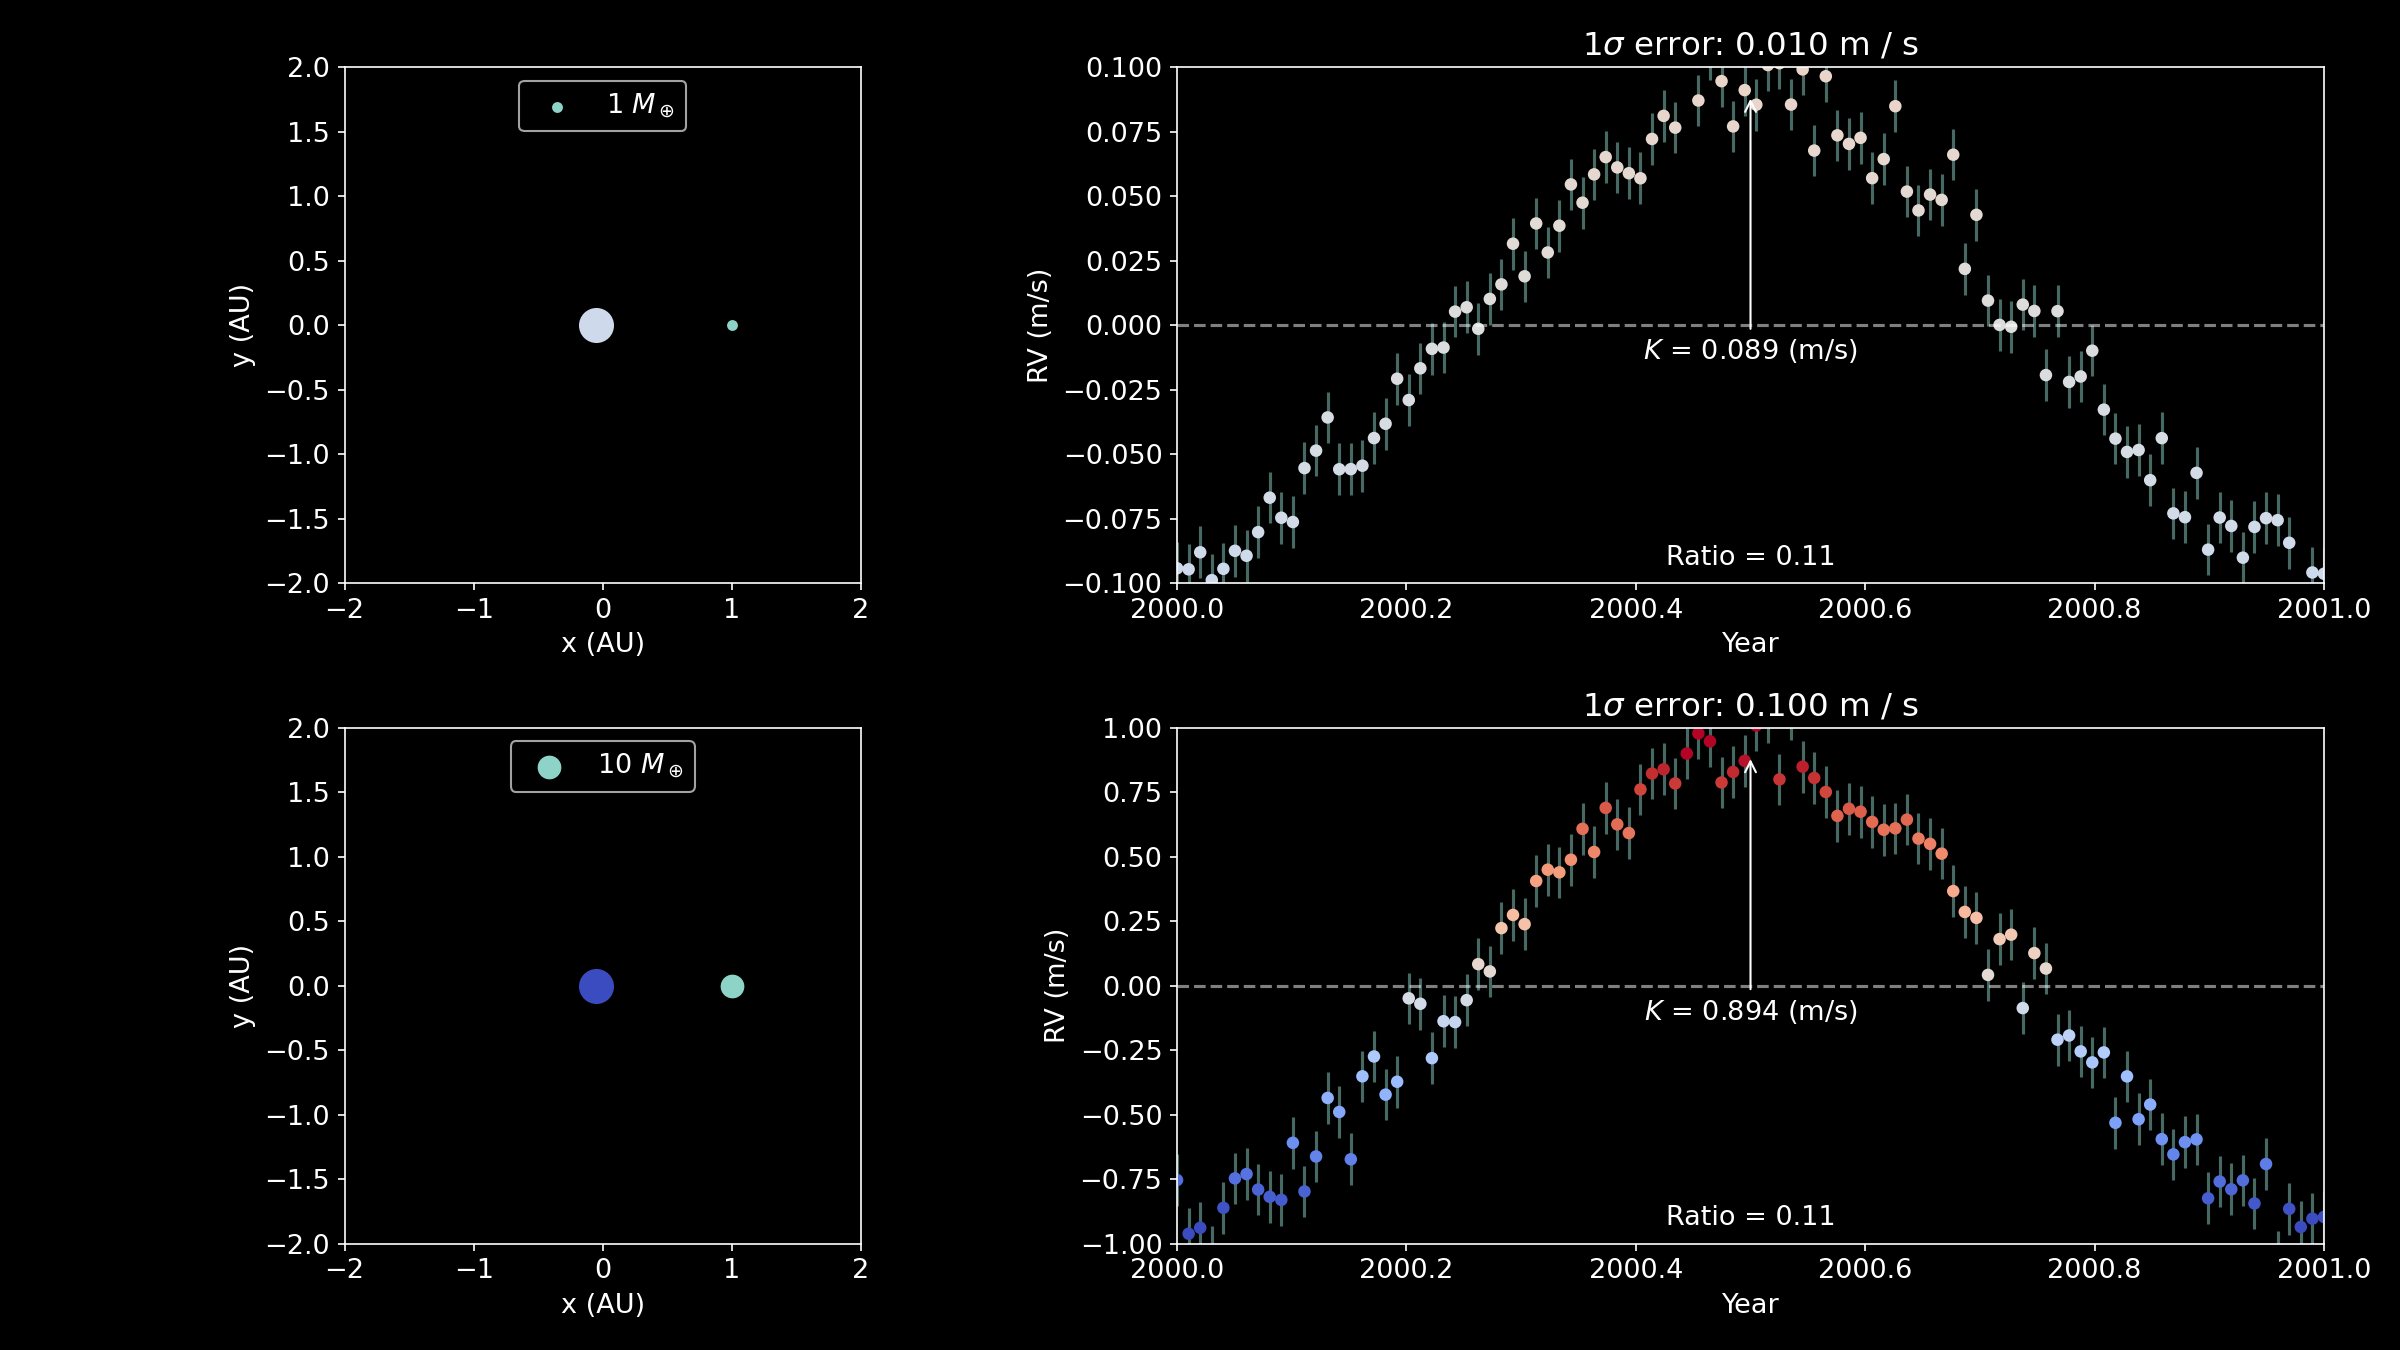
\includegraphics[width=12cm]{ratio_example/frame-99}
};
}

\frame{
    \frametitle{``True'' planet elements}
\tikzoverlay[text width = 14cm] at (0cm, 3cm+4.5pt){
    %\begin{itemize}
        %\item[\textbullet] Tested $1 \sigma $ errors of 0.1, 0.25, 0.5, 0.75, 1, 1.25, and 2 m/s
        %\item[\textbullet] RV semi-amplitude ($K$) fixed at 1 m/s
        %\item[\textbullet] Simple photometry with geometric albedo ($p$) fixed at Earth's 0.367
            %and Lambertian scattering
        %\item[\textbullet] Star distance ($d$) fixed at 10 parsecs
        %\item[\textbullet] Eccentricity ($e$) fixed at 0 (circular orbits)
        %\item[\textbullet] Inclinations ($i$) between 90 and 170 degrees
        %\item[\textbullet] Planet mass ($M_p$) calculated based on $K$ and $i$
        %\item[\textbullet] Planet radius ($R_p$) calculated based on $M_p$
        %\item[\textbullet] 10 linearly spaced semi-major axis ($a$) values between 1 and 2 AU
            %(orbital periods ($T$) between 365.25 and 1033.1 days)
    %\end{itemize}
    \begin{table}[htpb]
        \centering
        %\caption{caption}
        %\label{tab:label}
        \begin{tabular}{|c|c|c|}
            \hline
            \textbf{Parameter} & \textbf{Treatment} & \textbf{Value(s)} \\
            \hline
            $1 \sigma $ RV error & Varied & [0.1, 0.25, 0.5, 0.75, 1, 1.25, 2] m/s \\
            Inclination $i$ & Varied & Randomly sampled between [90, 170]$\degree$\\
            Semi-major axis $a$ & Varied & [1, 1.11, 1.22, \ldots, 2] AU\\
            \hline
            RV semi-amplitude $K$ & Fixed & 1 m/s \\
            Geometric albedo $p$ & Fixed & 0.367 \\
            Star distance $d$ & Fixed & 10 parsecs \\
            Eccentricity $e$ & Fixed & 0 (circular orbits) \\
            \hline
            Planet mass $M_p$ & Calculated & Calculated based on $K$ and $i$ \\
            Planet radius $R_p$ & Calculated & Calculated based on $M_p$\\
            \hline
        \end{tabular}
    \end{table}
    \begin{itemize}
        \item[\textbullet] Lambertian scattering for photometry
        \item[\textbullet] HabEx constraints, IWA of 0.058", OWA of 6", $\Delta \textrm{mag}_{0}$ of
            26.5
    \end{itemize}
};
}

\frame{
    \frametitle{Successful orbit construction}
\tikzoverlay[text width = 10cm] at (0cm-3pt, 2.6cm+4.5pt){
    \animategraphics[loop, controls, width=14cm]{100}{CI_if/ratio-0.50-frame-}{0}{364}
};
}

\frame{
    \frametitle{Failure modes}
\tikzoverlay[text width = 14cm] at (0cm, 3cm+4.5pt){
    \begin{itemize}
        \item[\textbullet] Identified two forms of failure
        \item[\textbullet] Intermittent failure, times when a mission scheduler would plan an
            observation with confidence even though the ``true'' planet is not detectable
        \item[\textbullet] Dispersion failure, when the orbits disperse so much that $P_{\textrm{det}}$
            flattens
    \end{itemize}
};
}

%\frame{
    %\frametitle{Intermittent failure}
%\tikzoverlay[text width = 14cm] at (0cm, 3cm+4.5pt){
%\begin{enumerate}
    %\item[1)] The true planet is not detectable;
    %\item[2)] The estimated probability of detection is in the top 90\% of the local probability of
        %detection values;
    %\item[3)] The probability of detection is changing by less than 0.0001 per day; and
    %\item[4)] The previous three conditions hold for 1 day.
%\end{enumerate}
%};
%}

\frame{
    \frametitle{Intermittent failure example}
\tikzoverlay[text width = 14cm] at (0cm, 3cm+4.5pt){
    \animategraphics[controls, width=14cm]{100}{ML_if/ratio-0.50-frame-}{0}{364}
};
}

\frame{
    \frametitle{Dispersion failure}
%\tikzoverlay[text width = 14cm] at (0cm, 3cm+4.5pt){
%\begin{enumerate}
    %\item[1)] Probability of detection curve flattens to the point where a full orbital period passes without any extrema
%\end{enumerate}
%};
\tikzoverlay[text width = 14cm] at (0cm, 3cm+4.5pt){
    \animategraphics[controls, width=14cm]{50}{CI_if/ratio-1.00-frame-}{0}{999}
};
%\includemedia[
  %width=0.9\linewidth,height=0.675\linewidth, %use this for embedded
  %%windowed=1000x500, %use this for floating window
  %activate=pageopen,
  %addresource=./figures/CI_if/output.mp4, %must be h.264 encoded
  %flashvars={
     %source=./figures/CI_if/output.mp4 
    %&autoPlay=true
    %&loop=true
%},
  %passcontext
%]{}{VPlayer.swf}
}

\frame{
    \frametitle{Full study results}
\tikzoverlay[text width = 9cm] at (-0.8cm, 3cm+4.5pt){
    \begin{itemize}
    \item[\textbullet] 20 years of propagation
    \item[\textbullet] ``No failure (always detectable)'' is not a useful metric
    \end{itemize}
    Conclusions
\begin{enumerate}
    \item[1)] Max KDE/Likelihood perform very poorly
    \item[2)] Credible interval slightly outperforms multivariate Gaussian at ratio of 0.1
    \item[3)] Multivariate Gaussian performs the best at ratios of 0.5 and above
    \item[4)] As variation in orbital elements increases (CI$>$MG$>$ML/KDE), the rate of dispersion failure increases
\end{enumerate}
};
\tikzoverlay[text width = 10cm] at (8.5cm-3pt, 3.5cm+4.5pt){
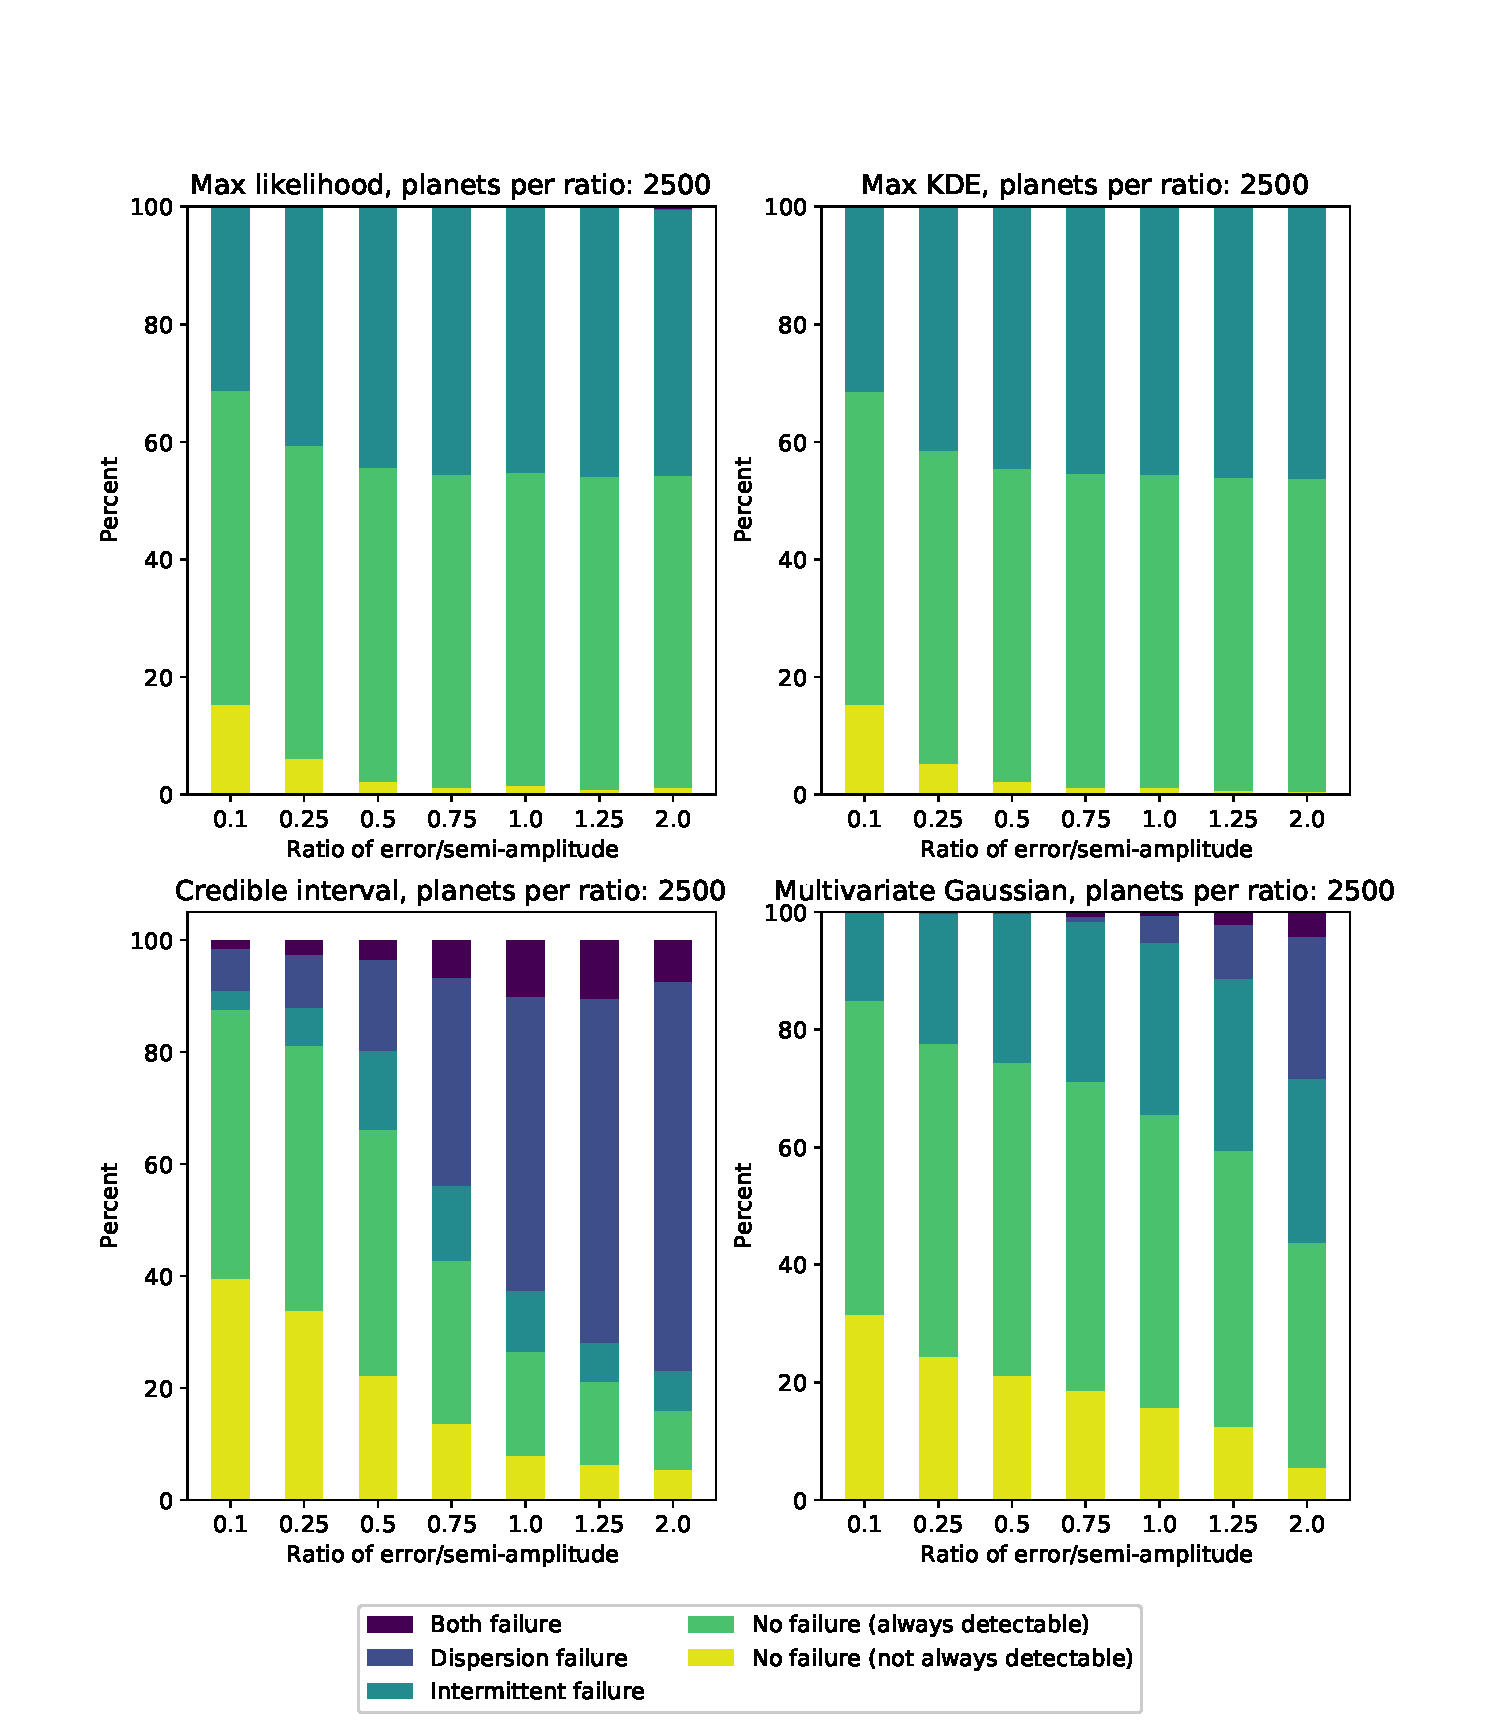
\includegraphics[height=8cm]{./figures/construction_method_bars_including_always_detectable.pdf}
};
}

%\frame{
    %\frametitle{Intermittent failure metrics}
%\tikzoverlay[text width = 14cm] at (-0.8cm, 3.2cm+4.5pt){
    %\begin{itemize}
    %\item[\textbullet] Intermittent failure can happen a single time or many during propagation
    %\item[\textbullet] Set up two metrics
        %\begin{enumerate}
            %\item[1)] Time of first intermittent failure, the time between start of propagation and the
                %first intermittent failure
            %\item[2)] Intermittent failure rate, the number of intermittent failures divided by the
                %number of time steps where the true planet is not detectable
        %\end{enumerate}
    %\end{itemize}
%};
%TODO create graphic with the different metrics labeled
%}
\frame{
    \frametitle{Intermittent failure results}
\tikzoverlay[text width = 10cm] at (1.1cm-3pt, 3.1cm+4.5pt){
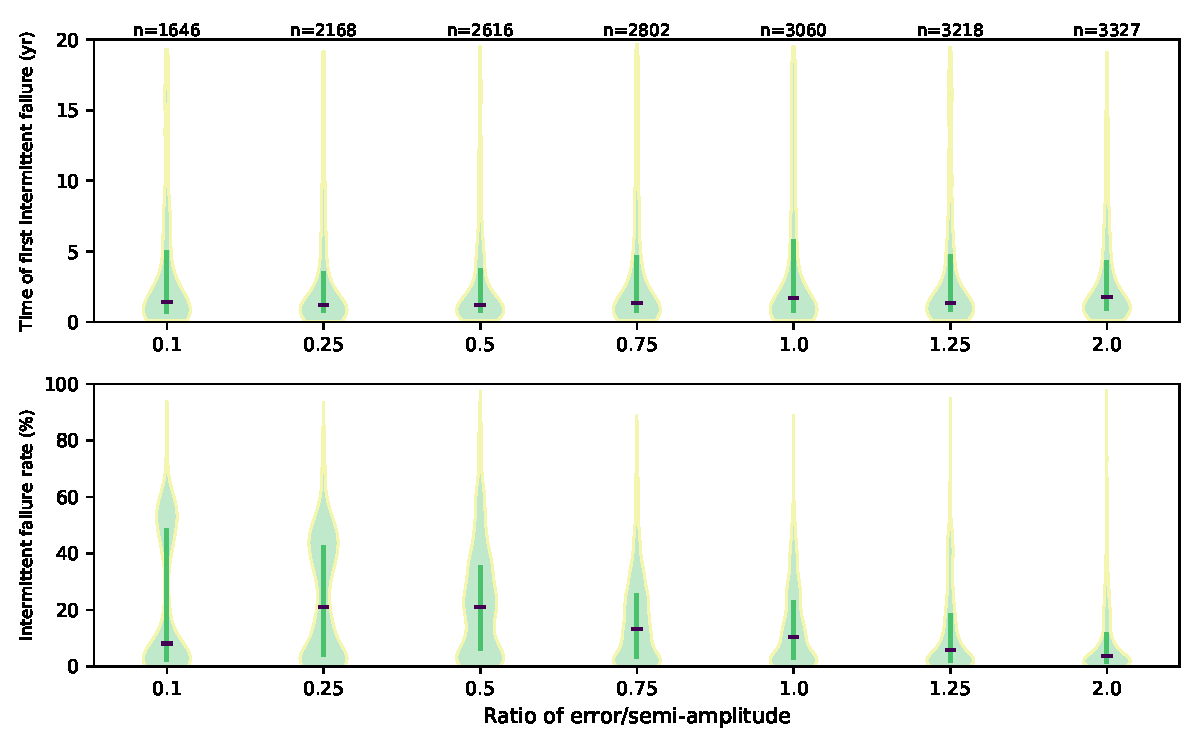
\includegraphics[height=7.5cm]{./figures/violin_plots.pdf}
};
}

\frame{
    \frametitle{Summary of work}
    \begin{enumerate}
        \item[1)] Identified 4 methods of constructing orbits from RV fit information
        \item[2)] Trade off between intermittent and dispersion failure
        \item[3)] Using a single set of orbital elements performs poorly
        \item[4)] For low ratios more variation in orbital elements is prefered
        \item[5)] For medium ratios (0.5 and up) multivariate Gaussian performs the best
        \item[6)] In cases with intermittent failure, it is overwhelmingly likely to happen within a
            few orbital periods
        \item[7)] At low ratios orbit construction that creates intermittent failure is more damaging than
            at higher ratios
    \end{enumerate}
}

%%%%%%%%%%%%%%%%%%%%%%%%%%%%%%%%%%%%%%%%%%%%%%%%%%%%%%%%%%%%%%%%%%%%%%%%%%%%%%%%%%%%%%%%%%%%%

\section{Future work}
\subsection{Future work}
\frame{
\frametitle{Generalize the multivariate Gaussian}
\begin{itemize}
    \item[\textbullet] Want to adapt it to increase variation as the ratio decreases
    \item[\textbullet] Expect that to improve performance at low ratios (similar to credible
        interval)
\end{itemize}
}

\frame{
\frametitle{Improved photometry}
\begin{itemize}
    \item[\textbullet] Run simulations with more realistic photometry
        \begin{enumerate}
            \item[1)] Classify planets using Kopparapu bins \parencite{Kopparapu2018b}
            \item[2)] Use different photometry calculations based on planet classification, likely
                the color classification grid from \textcite{Batalha2018a} for Jovian planets,
                unsure of reliable rocky planet photometry model
            \item[3)] Run the failure mode analysis again
        \end{enumerate}
\end{itemize}
}

\frame{
\frametitle{Precursor RV target optimization and validation}
\begin{itemize}
    \item[\textbullet] Create EXOSIMS SimulatedUniverse module that provides synthetic RV data that can be
        fitted with RadVel
    \item[\textbullet] Implement the multivariate Gaussian construction method in EXOSIMS
    \item[\textbullet] Use the $P_{\textrm{det}}$ metric in the target list cost function and
        simulate missions to see the effect of this procedure on exoplanet yield
\end{itemize}
}

\frame{
\frametitle{Multi-planet RV signals}
\begin{itemize}
    \item[\textbullet] Set up this process to work with planetary systems with multiple planets
    \item[\textbullet] Would need to study the problem of identifying how many planets make up the
        RV curve
    \item[\textbullet] Might require a number of major assumptions to simulate more detailed
        analysis than can be automated (i.e. assume I already know the number of planets before
        fitting with RadVel)
\end{itemize}
}

%%let's make an appendix with refs and backup slides
%we don't want to count these in the slide total, so we'll stop counting here
\newcounter{finalframe}
\setcounter{finalframe}{\value{framenumber}}

\appendix
\frame{
    \frametitle{Contributions}
    \begin{scriptsize}
    Journal Publications:
    \begin{itemize}
        \item[\textbullet] Spohn C, et al. (2021) ``Scheduling direct imaging observations based on
            radial velocity orbit fits'' The Astronomical Journal (In review)
        \item[\textbullet] Keithly D, et al. (2021) ``Integration time adjusted completeness'' JATIS
        \item[\textbullet] Ahmadi F, et al. (2020) ``Suppressing Condensation Frosting
            Using an Out-of-Plane Dry Zone'' Langmuir
    \end{itemize}
    Conference Presentations:
    \begin{itemize}
        \item[\textbullet] Spohn C, et al. (2020) ``How orbital fit uncertainties impact dynamic scheduling
            '' SPIE (Paper and poster)
        \item[\textbullet] Spohn C, et al. (2020) ``From RV to Direct Imaging: How RV Fits Degrade''
            Roman CGI Symposium (Presentation)
        \item[\textbullet] Spohn C, et al. (2020) ``Dynamically Scheduling Direct Imaging Missions''
            AAS (Poster)
        \item[\textbullet] Spohn C, et al. (2019) ``Orbital Error Propagation for Direct Detection''
            ERES (Poster)
        \item[\textbullet] Spohn C, et al. (2017) ``A Bridge Too Far: Suppressing Frost Using an
            Out-of-Plane Dry Zone'' APS DFD (Presentation)
        \item[\textbullet] Spohn C, et al. (2017) ``3d Printing Icicles with Evaporating Droplets'' APS DFD (Poster)
    \end{itemize}
    Code contributions
    \begin{itemize}
        \item github.com/dsavransky/EXOSIMS
        \item github.com/dsavransky/plandb.sioslab.com
    \end{itemize}

\end{scriptsize}
}


\frame{
    \frametitle{Coursework}

}

\frame{
    \frametitle{Acknowledgements}

}
{
\subsection{References}
\frame[allowframebreaks]{
\frametitle{References}
\printbibliography  
}}

%%backup slides:
\section{Backup}
\subsection{Backup}

\frame{
\frametitle{Completeness, $C$}
\tikzoverlay[text width = 6cm] at (0cm, 2.5cm+4.5pt){
\begin{enumerate}
    \item[\textbullet] Simulation based metric that calculates the probability of detecting a planet around a target
        star, should a planet in the assumed population exist
    \item[\textbullet] With enough simulated planets $C$ is constant
    \item[\textbullet] Useful when there are no prior detections around a star
\end{enumerate}
\begin{align*}
    C = \frac{\textrm{\# of detectable simulated planets}}{\textrm{\# of simulated planets}}
\end{align*}
};
\tikzoverlay[text width = 7cm] at (7cm, 3.1cm+4.5pt){
    \animategraphics[loop, controls, width=7cm]{10}{completeness/frame-}{0}{9}
};
\footlineextra{\textcite{Brown2004c}, \textcite{Brown2005d}, \textcite{Garrett2016}}
}
\frame{
\frametitle{Completeness, $C$}
\tikzoverlay[text width = 12cm] at (0cm, 3.1cm+4.5pt){
    \animategraphics[loop, controls, width=14cm]{10}{comp_constraint/frame-}{0}{9}
};
}

\frame{
    \frametitle{Intermittent failure}
\tikzoverlay[text width = 14cm] at (0cm, 3cm+4.5pt){
\begin{enumerate}
    \item[1)] The true planet is not detectable;
    \item[2)] The estimated probability of detection is in the top 90\% of the local probability of
        detection values;
    \item[3)] The probability of detection is changing by less than 0.0001 per day; and
    \item[4)] The previous three conditions hold for 1 day.
\end{enumerate}
};
}

\frame{
    \frametitle{Intermittent failure metrics}
\tikzoverlay[text width = 14cm] at (-0.8cm, 3.2cm+4.5pt){
    \begin{itemize}
    \item[\textbullet] Intermittent failure can happen a single time or many during propagation
    \item[\textbullet] Set up two metrics
        \begin{enumerate}
            \item[1)] Time of first intermittent failure, the time between start of propagation and the
                first intermittent failure
            \item[2)] Intermittent failure rate, the number of intermittent failures divided by the
                number of time steps where the true planet is not detectable
        \end{enumerate}
    \end{itemize}
};
%TODO create graphic with the different metrics labeled
}

%\frame[label=backup1]{
%\frametitle{A Backup Slide with Additional Info}
%\framesubtitle{ \hyperlink{mainslide1}{\beamerreturnbutton{Return}} }
%Lots of nitty-gritty stuff that doesn't belong in the main talk
%}


%\setcounter{framenumber}{\value{finalframe}} %reset the counter

\end{document}
